% !TEX root = report.tex

\section{Results}
\label{sec:results}
% Dazzling numerical results

\subsection{Performance measure}

% \subsubsection{F-Score}

The F-Score is a metric that combines the values of precision and recall to
provide an estimate of the quality of the predictions made on a test dataset.
Precision is the fraction of relevant data among the selected instances, the
number of true positives over all the samples selected (a high precision score
means that there are few false positives).
% MAYBE how confident you are that a selected is really in that class.
Recall is the fraction of selected instances among all the relevant samples,
the number of true positives over all the true samples (a high recall score
means that there are few false negatives). The F-Score is obtained as the
harmonic mean of precision and recall.

% Confusion matrix
Another tool used to visually show the performance of a model
is the confusion matrix, that is closely related to the F-Score.
The predicted labels are listed on the x-axis,
the real labels are listed on the y-axis.
% On the x-axis the predicted labels are listed,
% on the y-axis the real labels are listed.
The confusion matrix contains
the number of occurences
for each combination of predicted/real labels.
The main diagonal contains the correctly identified samples.
Along the rows there are the false negatives for a label,
and along the columns there are the false positives for a label.

% \subsubsection{Graphs}

Throughout this section, several groups of graphs will be shown, that present
at once the F-score value for combinations of up to four hyper-parameters.
For example, say there is a graph 
with title 
``paramA: valueA, paramB: [valuesB]
grouped by paramC: [valuesC]
grouped by paramD: [valuesD]''.
This graph is part of a group of graphs, where the value of the first parameter
(valueA) is fixed for each sub-graph.
The other three parameters vary within the sub-graph:
% each packet of columns shows the variation of the parameter B,
% whose values are shown in the legend.
within each group of column the parameter B is changing,
whose values are shown in the legend.
% The groups of columns show the variation of the parameter C,
% whose values are shown as labels of the x axis.
% Each super group of columns show the variation of the parameter D,
% whose values are shown between parenthesis as labels of the x axis.
The other two parameters vary for each group of columns:
the values are indicated in the label of the x axis as ``valueC (valueD)''.
The other hyper-parameters are averaged for each column.
% , within reason:
% Average the others within reason (eg only one type of task).
The height of the column shows the mean F-score value for that
combination of parameters,
the black line indicates the min/max values of F-score and the
blue line tells the standard deviation around the mean.

\subsection{Hyper-parameter analysis: CNN}

% \subsection{Hyper-parameter analysis}
% Hypa comparison
% First specific hypas

A total of $5064$
% TODO
experiment were performed for the convolutional architecture.

\subsubsection{Model parameters performance comparison}

The effects of tweaking the parameters of the model structure are shown in
\fig{fig:cnn_comparison_kernel_filter_dense_pool}.
The graph sums up the F-Score values for variation of
a)
the number of convolutional filters learned,
b)
the shape of the filters ($01$ for square kernel sizes, $02$ for a vertical
filter followed by two square filters),
c)
the shape of the pooling window ($01$ for square, $02$ for a rectangular
window followed by two square ones)
and
d)
the number of units in the dense classifier.
% clear see kernel
% clear see dense
% pool vague
% filter useless
% Fscore__kernel_size__filters__dense_width__pool_size.png
Several insights can be extrapolated, in order of clarity:
\begin{itemize}
    \item The vertical kernel helps extract information along the frequency axis,
        and provides a clear increase in performance.
    \item A larger dense classifier leads to better performance,
        that saturates at $64$, and further increase does not help.
    \item A high number of filter is not needed to achieve a good performance,
        any value larger than $10$ performed equally well, from $20$ to $128$.
    \item Square pool windows perform slightly better than the rectangular ones.
\end{itemize}

% TODO: on what is averaged

\begin{figure*}[h!]
    \centering
    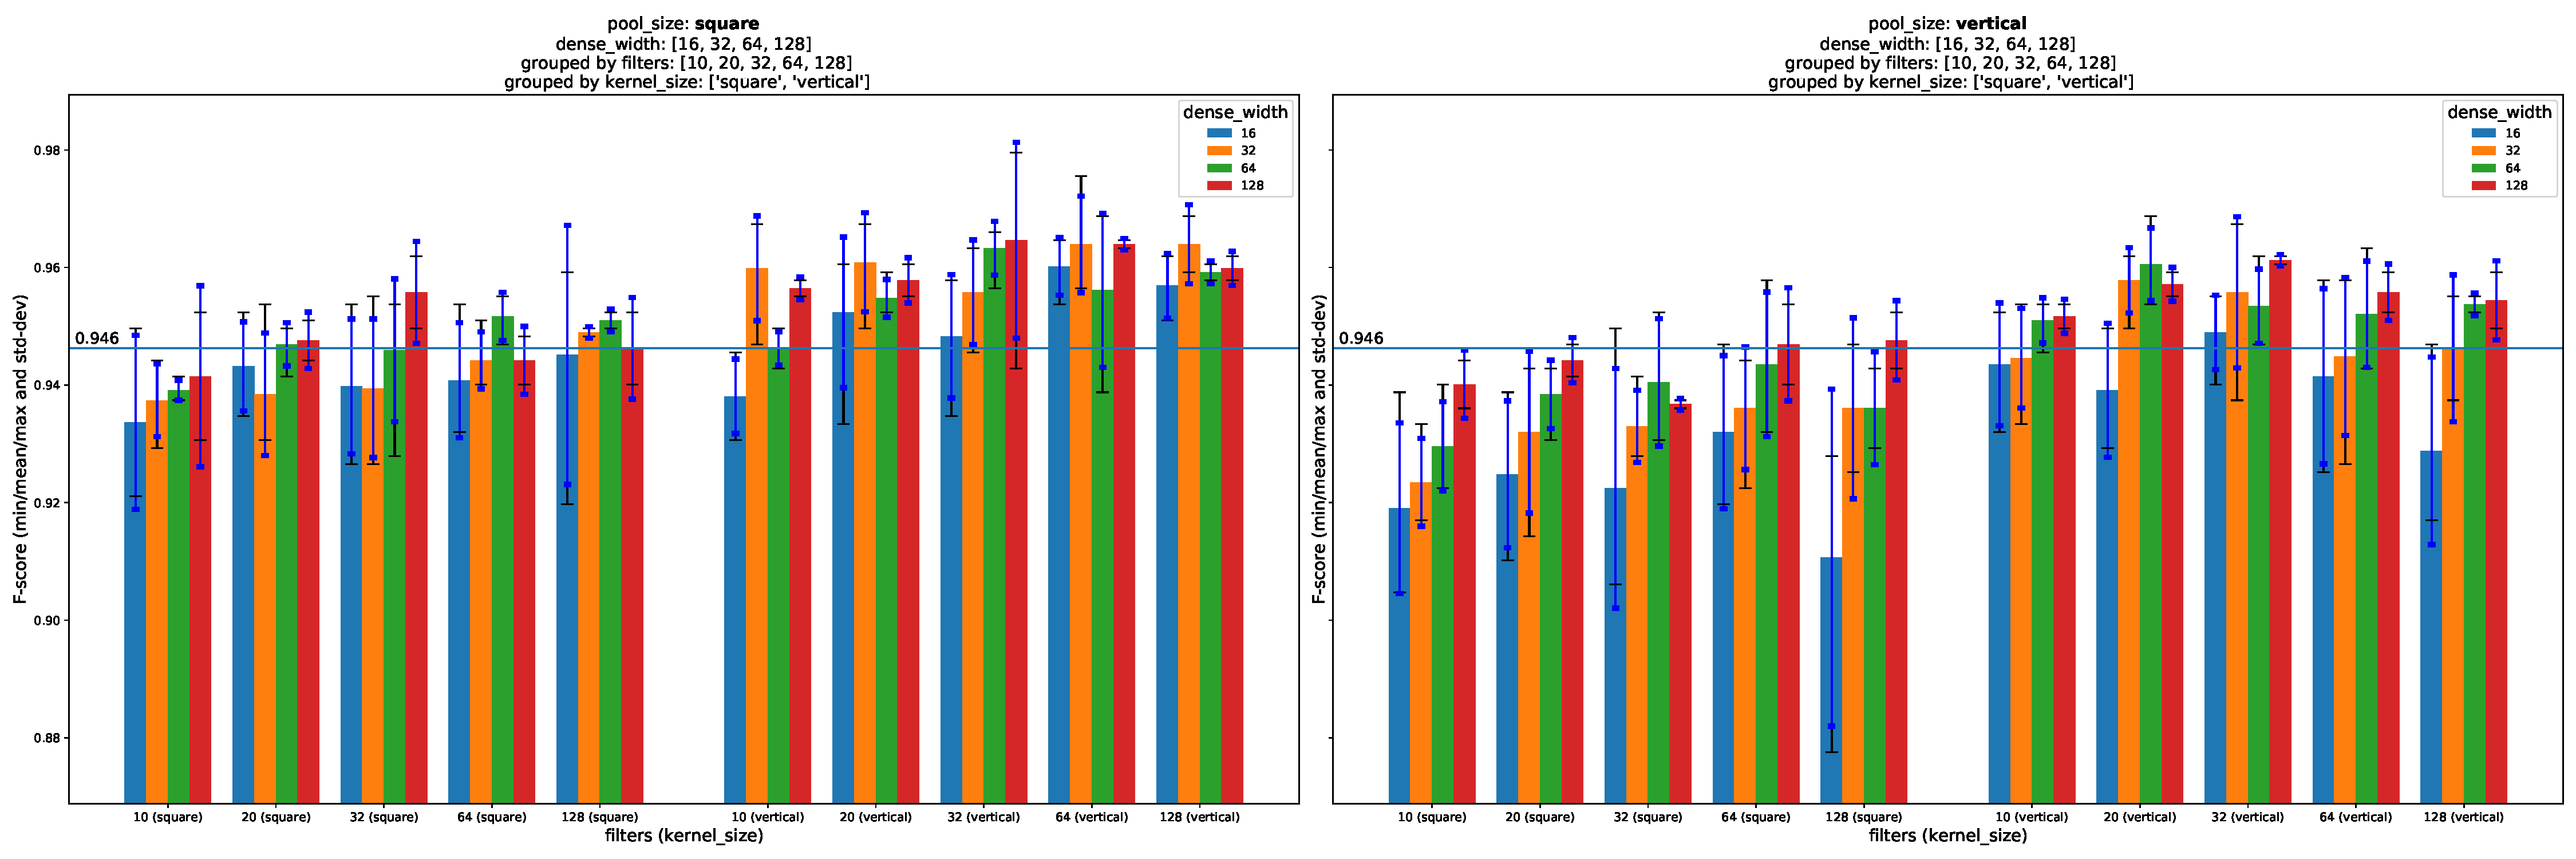
\includegraphics[width=0.9\linewidth]{Fscore_CNN_kernel_size__filters__dense_width__pool_size.pdf}
    \caption{Comparison CNN model}%
    \label{fig:cnn_comparison_kernel_filter_dense_pool}
\end{figure*}

\subsubsection{Training parameters performance comparison}

\fig{fig:cnn_comparison_epoch_lr_dataset} shows F-Score values for
variation of
the dataset used (MFCC spectrogams, mel sectrograms, agumented mel spectrogams)
and the learning rate used (fixed or with exponential decay).
Two main conclusions can be reached:
\begin{itemize}
    \item 
        Mel Frequency Cepstral Coefficients are clearly outperformed by mel
        spectrograms, as expected, considering that the MFCC are built to be composed
        by uncorrelated vectors, so interpreting the input as an image is not
        recommended.
        The benefit of augmentation are less clear, more details are provided
        in \secref{sec:augmentation_performance} and
        \tab{tab:augmentation_comparison_performance}.
    \item 
        The first three packets of columns correspond to fixed learning rate values,
        while the last three correspond to an exponential decay schedule.
        An increase in performance is achieved with the exponential schedules.
\end{itemize}

\begin{figure*}[h!]
    \centering
    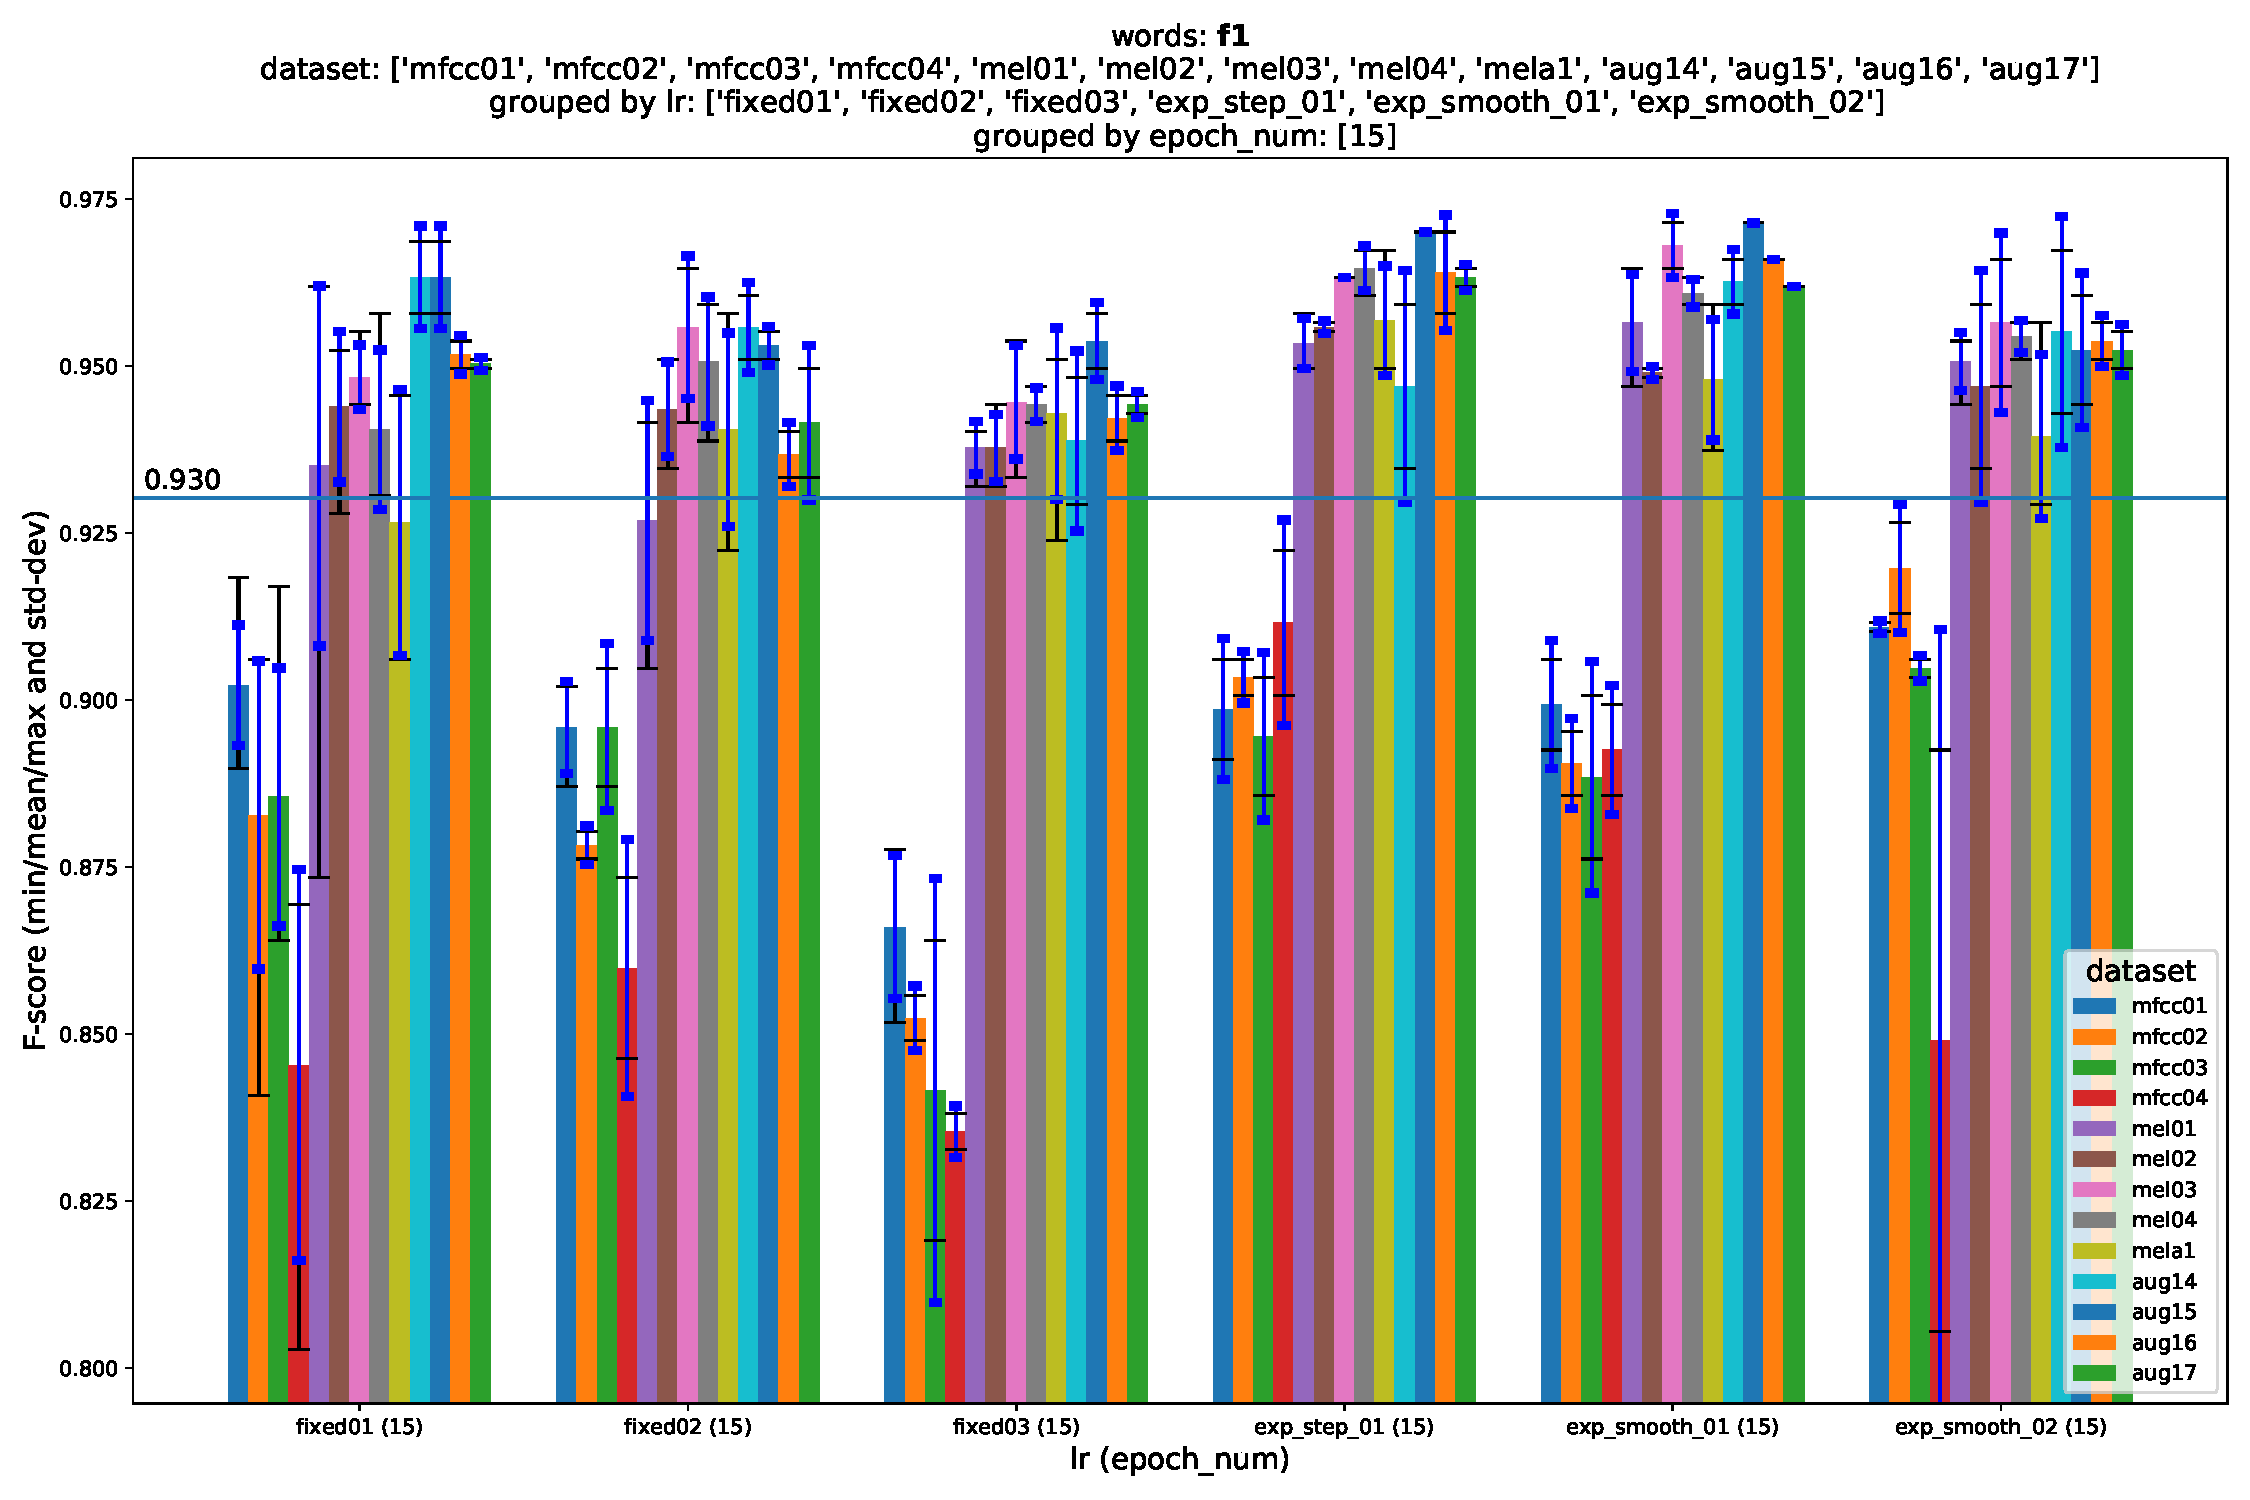
\includegraphics[width=0.9\linewidth]{Fscore_CNN_epoch_num__lr__dataset__words.pdf}
    \caption{Comparison CNN}%
    \label{fig:cnn_comparison_epoch_lr_dataset}
\end{figure*}

\subsection{Hyper-parameter analysis: Transfer learning}

A total of $144$
% TODO
experiment were performed for the transfer learning approach.

% TODO: on what are you averaging

\subsubsection{Model and training parameters performance comparison}

\fig{fig:tra_comparison_batch_epoch_dense} shows the effects of tuning
a)
the number of training epochs
b)
the number of samples per batch
c)
the shape of the final classifier built on top of the Xception model.
% Fscore__batch_size__epoch_num__dense_width__words.png
Using a combination of $[40, 20]$ epochs and $[16, 16]$ as batch sizes seems to
achieve the best performance, while the shape of the classifier does not
influence the training.

% Fscore_TRA_batch_size__epoch_num__dense_width__words.pdf

\begin{figure}[h!]
    \centering
    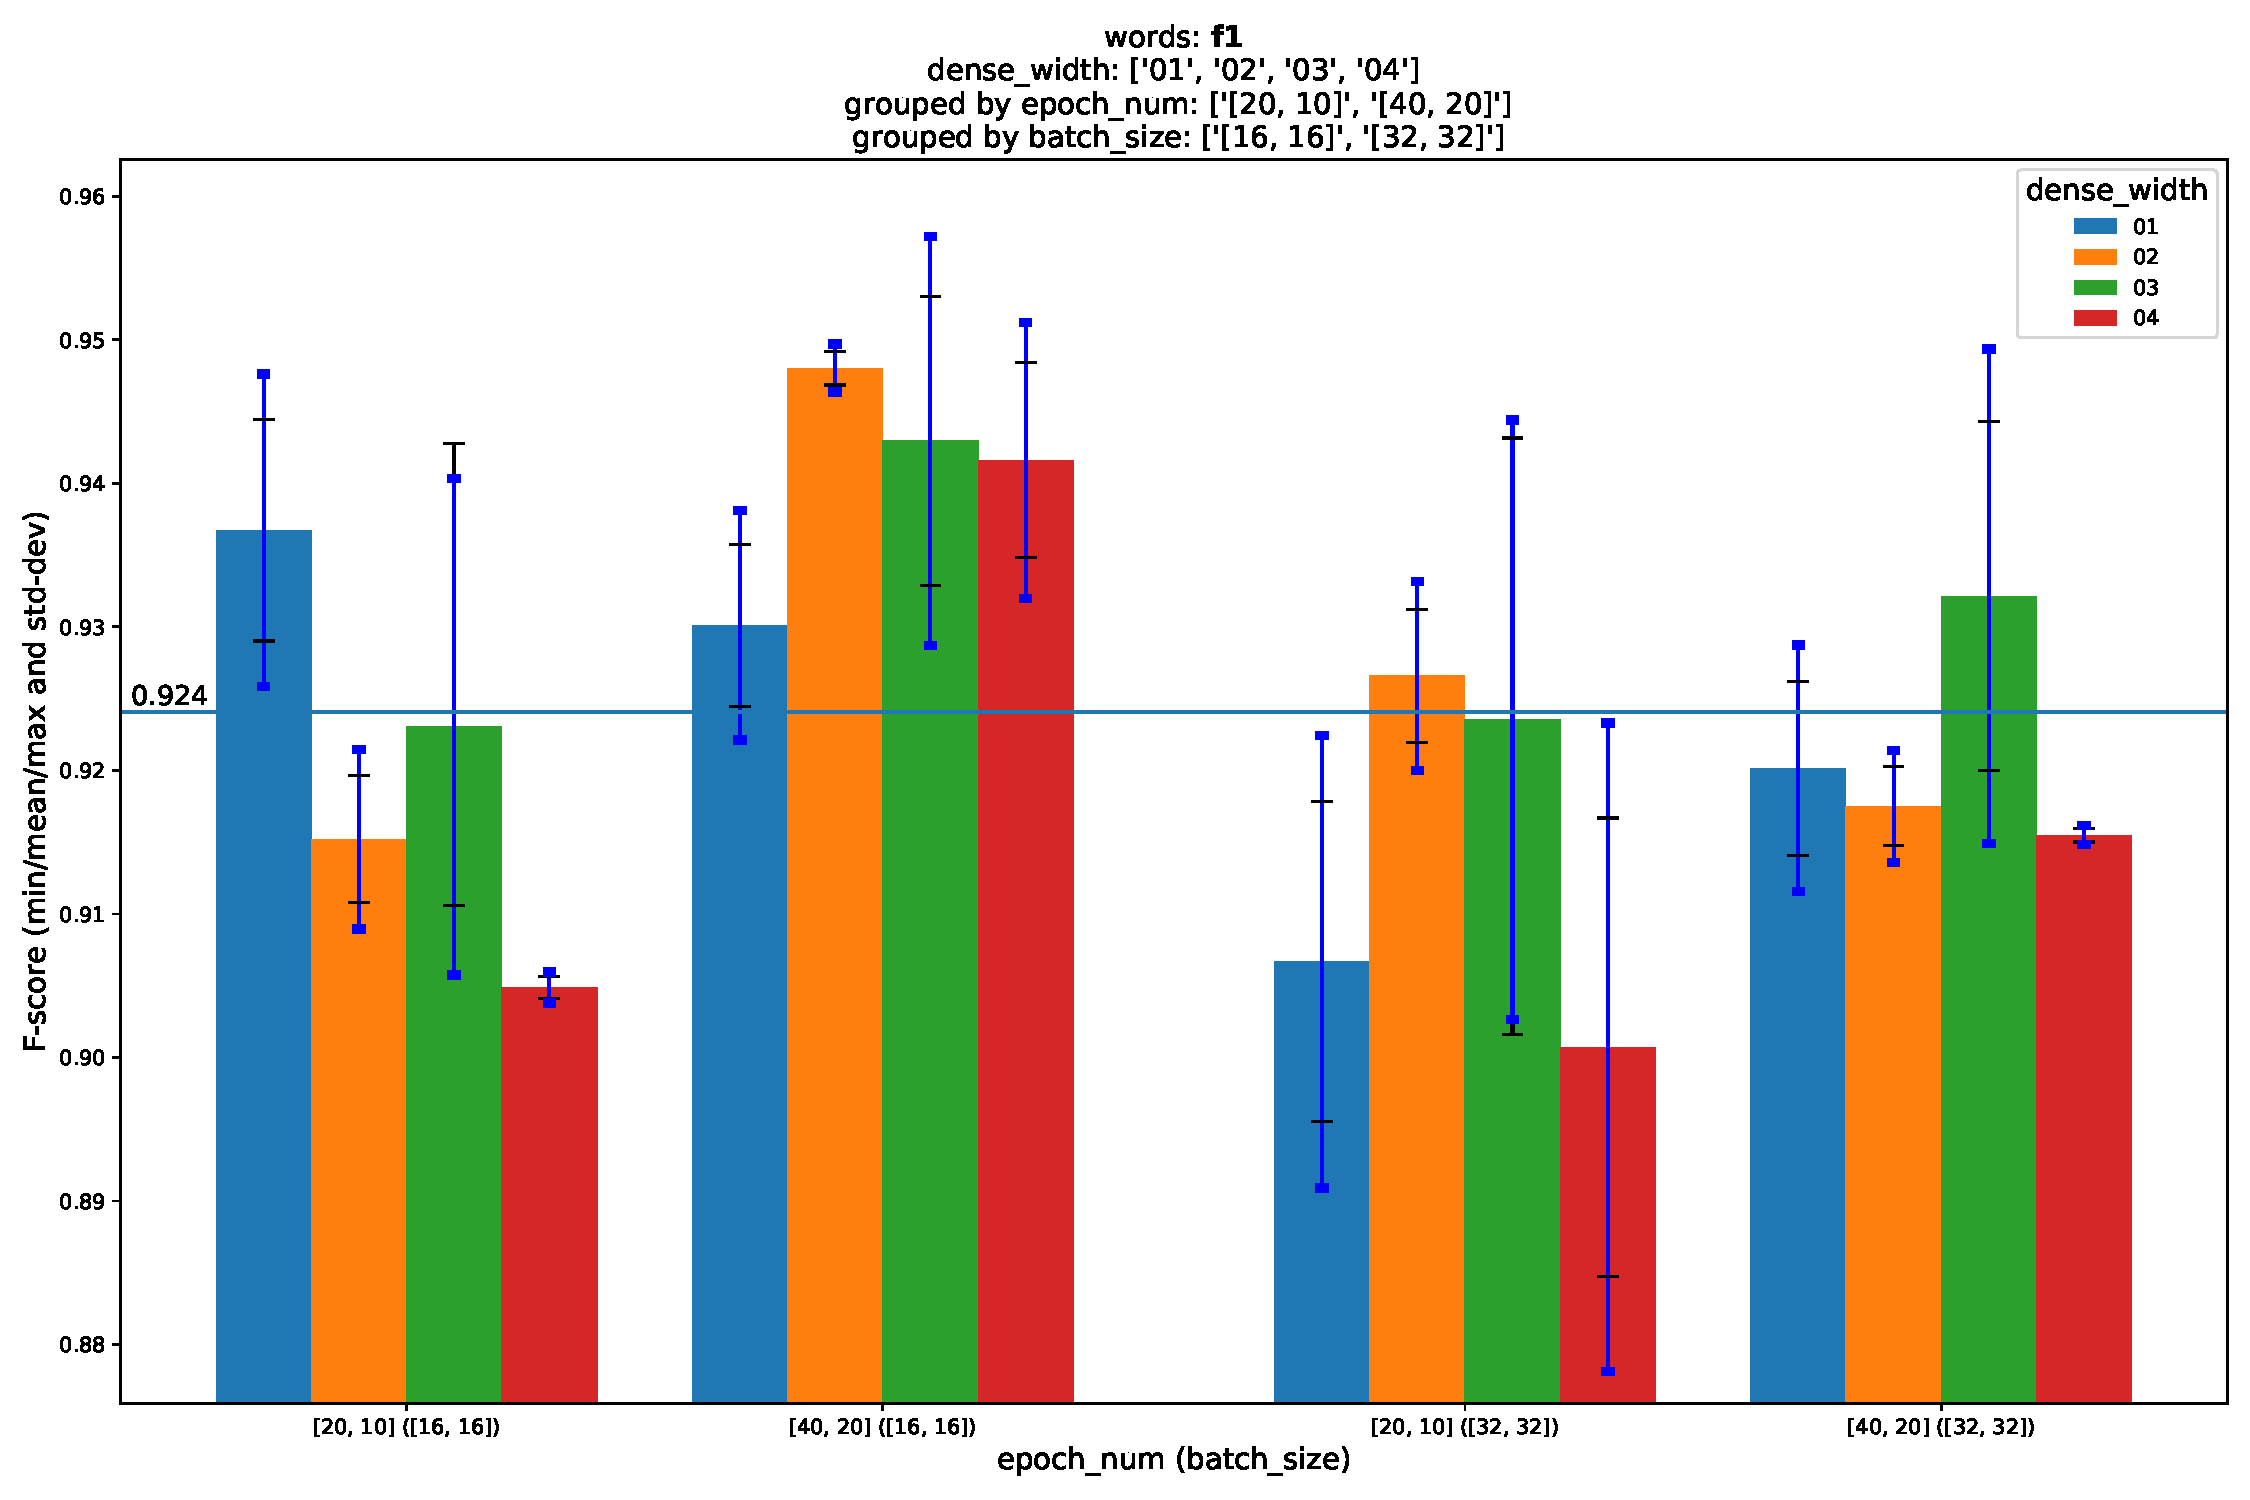
\includegraphics[width=0.8\linewidth]{Fscore_TRA_batch_size__epoch_num__dense_width__words.pdf}
    \caption{TRA comparison batch epoch dense}%
    \label{fig:tra_comparison_batch_epoch_dense}
\end{figure}

\subsubsection{Dataset performance comparison}

\fig{fig:tra_comparison_dataset}

% TODO: what are you averaging?

The different ways used to stack the spectrograms to obtain a 3-channels image
are compared in \fig{fig:tra_comparison_dataset}.
Stacking 128x128 mel spectrograms works quite well, as expected.
Similarly, stacking three mel spectrograms obtained by composing two 128x64
spectrograms each, can lead to similar results.
The MFCC spectrograms do not work as well, just as seen with the small
convolutional networks.
All these images had uniform structure across the depth dimension, as they were
obtained by stacking spectrograms with the same shape and type.
However, reasonably good results are also obtained by stacking spectrograms of
different kinds: both stacking 2 mel and 1 MFCC and stacking 1 mel, 1 MFCC and
1 composed.
In these last two types, there is little cross-channel correlation.
Considering that the base model used is Xception, that learns independently the
spatial and cross-channel correlations, it makes sense that the results are
decent, as the model learns to exploit the spatial correlations, but some
performance is lost as there is no information to be extracted by the
cross-channel correlations between different types of spectrograms.

\begin{figure}[h!]
    \centering
    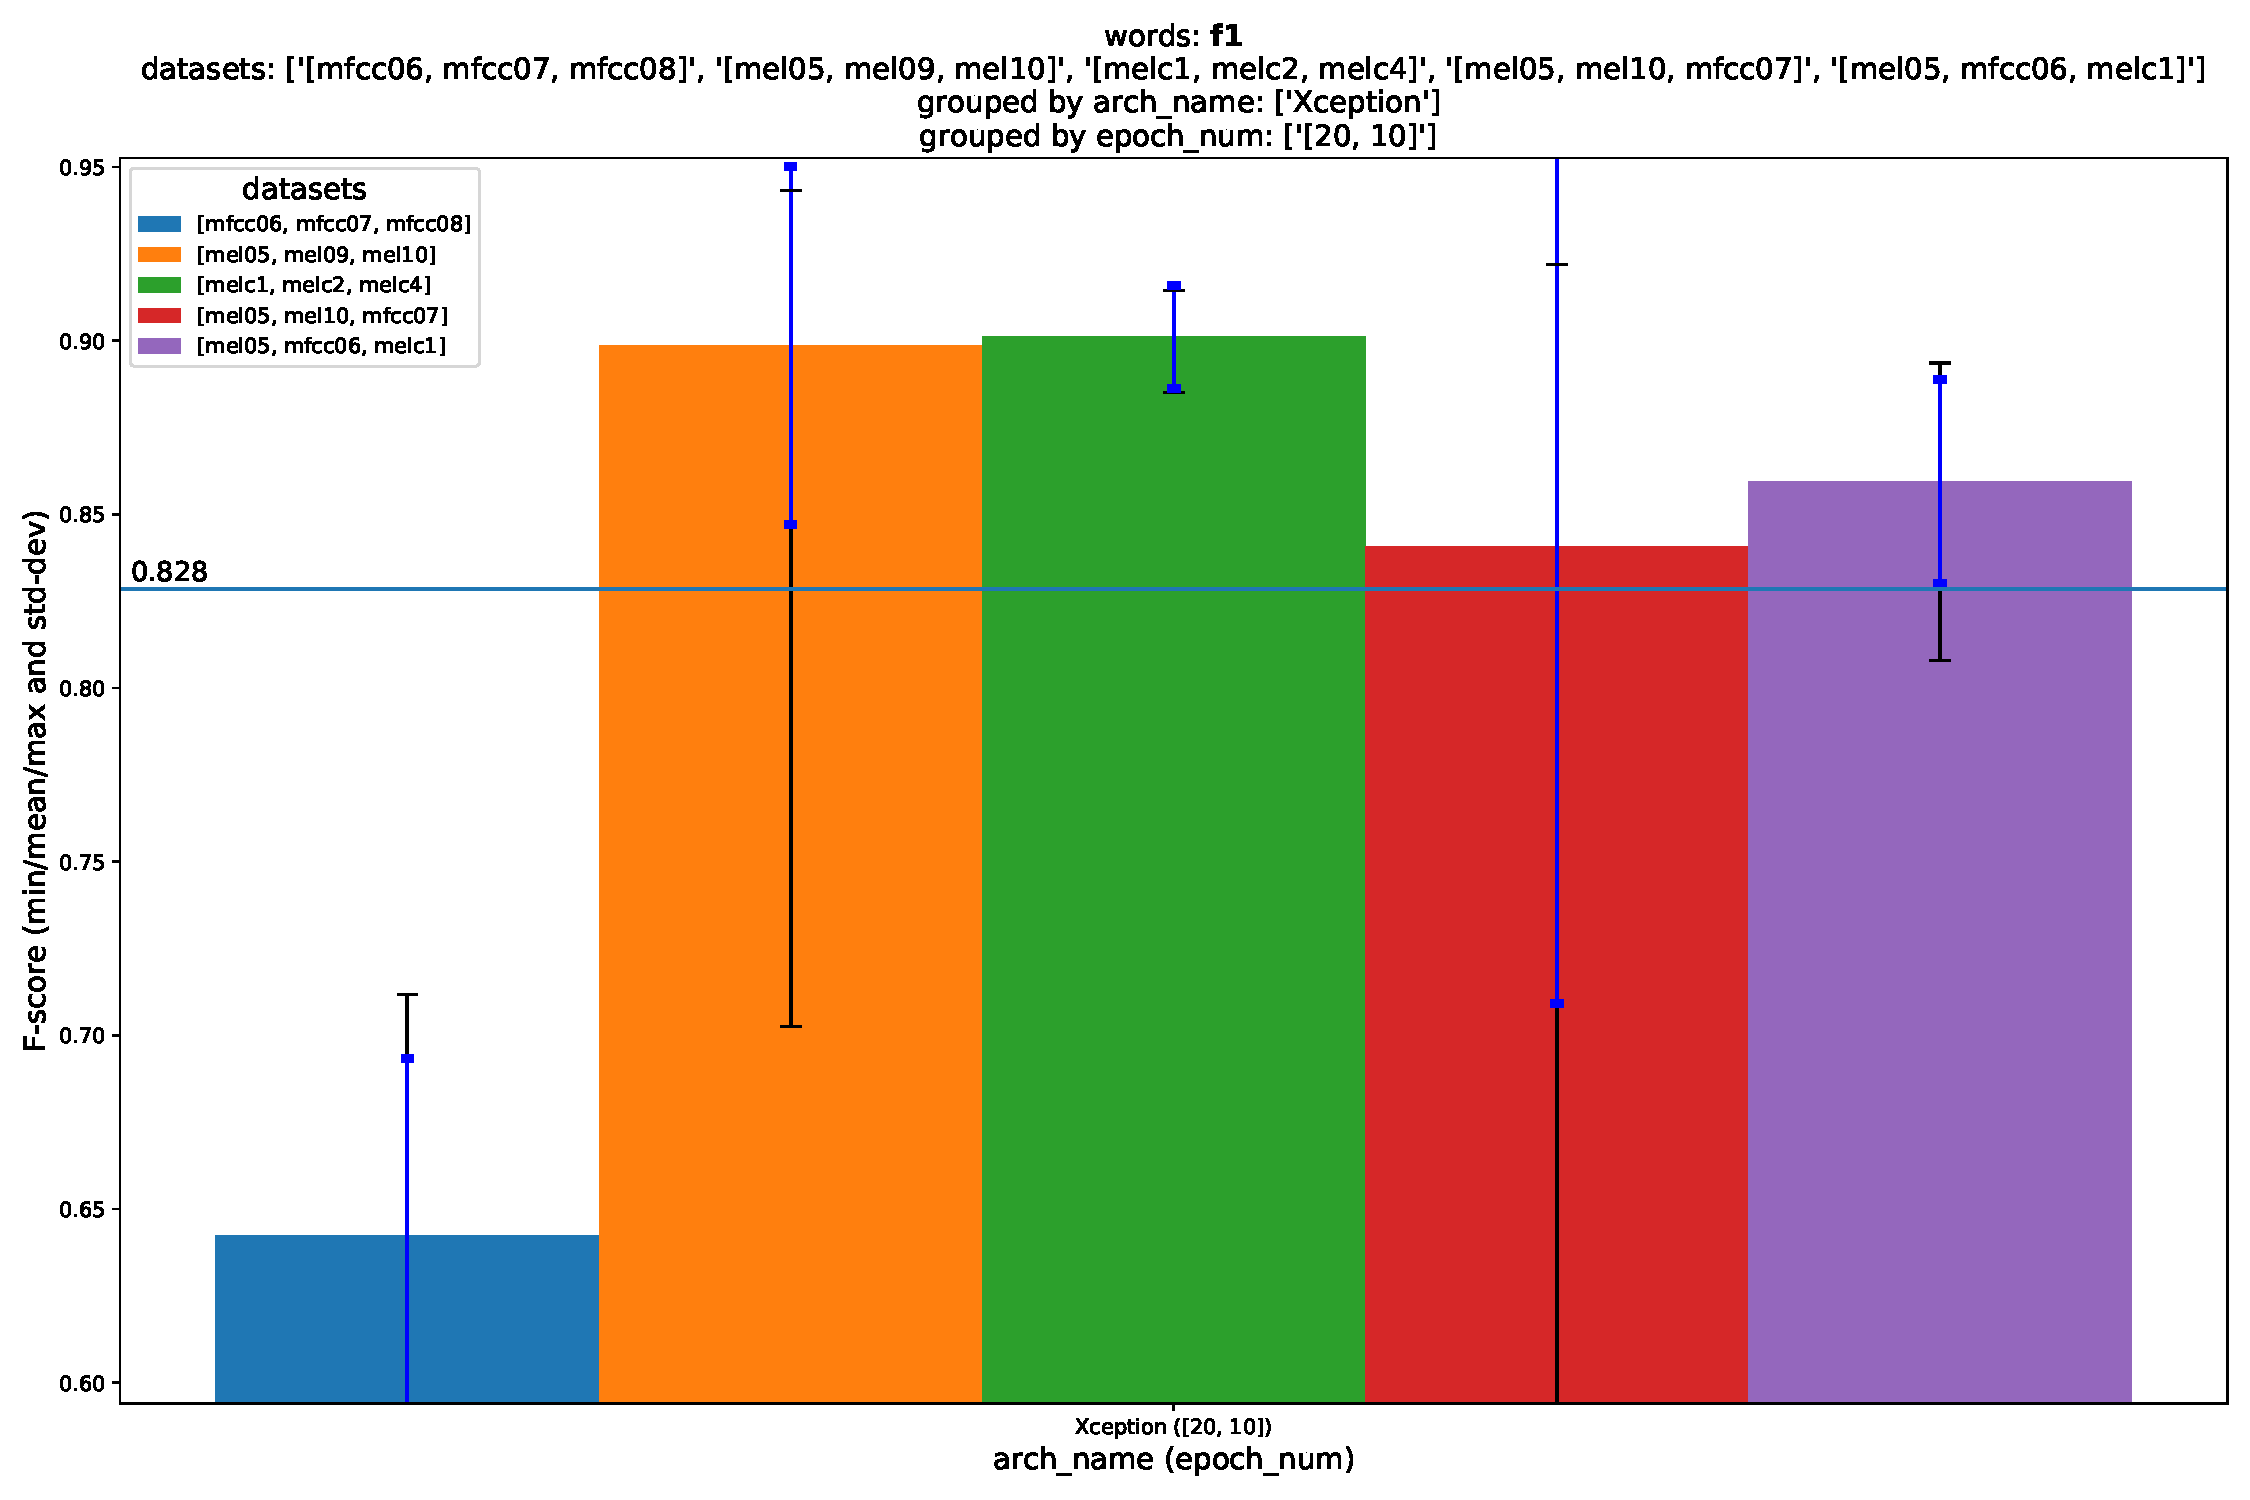
\includegraphics[width=0.8\linewidth]{Fscore_TRA_dataset_comparison.pdf}
    \caption{Dataset TRA comparison}%
    \label{fig:tra_comparison_dataset}
\end{figure}

\subsubsection{Architecture performance comparison}


\fig{fig:tra_comparison_arch} shows the performances of different base models:
The best model architectures are DenseNet121 and EfficientNetB7.
It is worth noting that the latter is a far larger network, as DenseNet121 only
has 7M parameters compared to the 66M of EfficientNetB7.
EfficientNetB4 also achieves very good results, using only 19M parameters,
outperformimg by a little Xception, with 22.8M parameters.
EfficientNetB0, with 5.3M parameters, cannot reach the same results.

% TODO: EfficientNet exactly like in the paper the nice curve precision vs number params

% 7M DenseNet121
% 22.8M Xception
% 5.3M B0
% 19M B4
% 66M B7

\begin{figure}[h!]
    \centering
    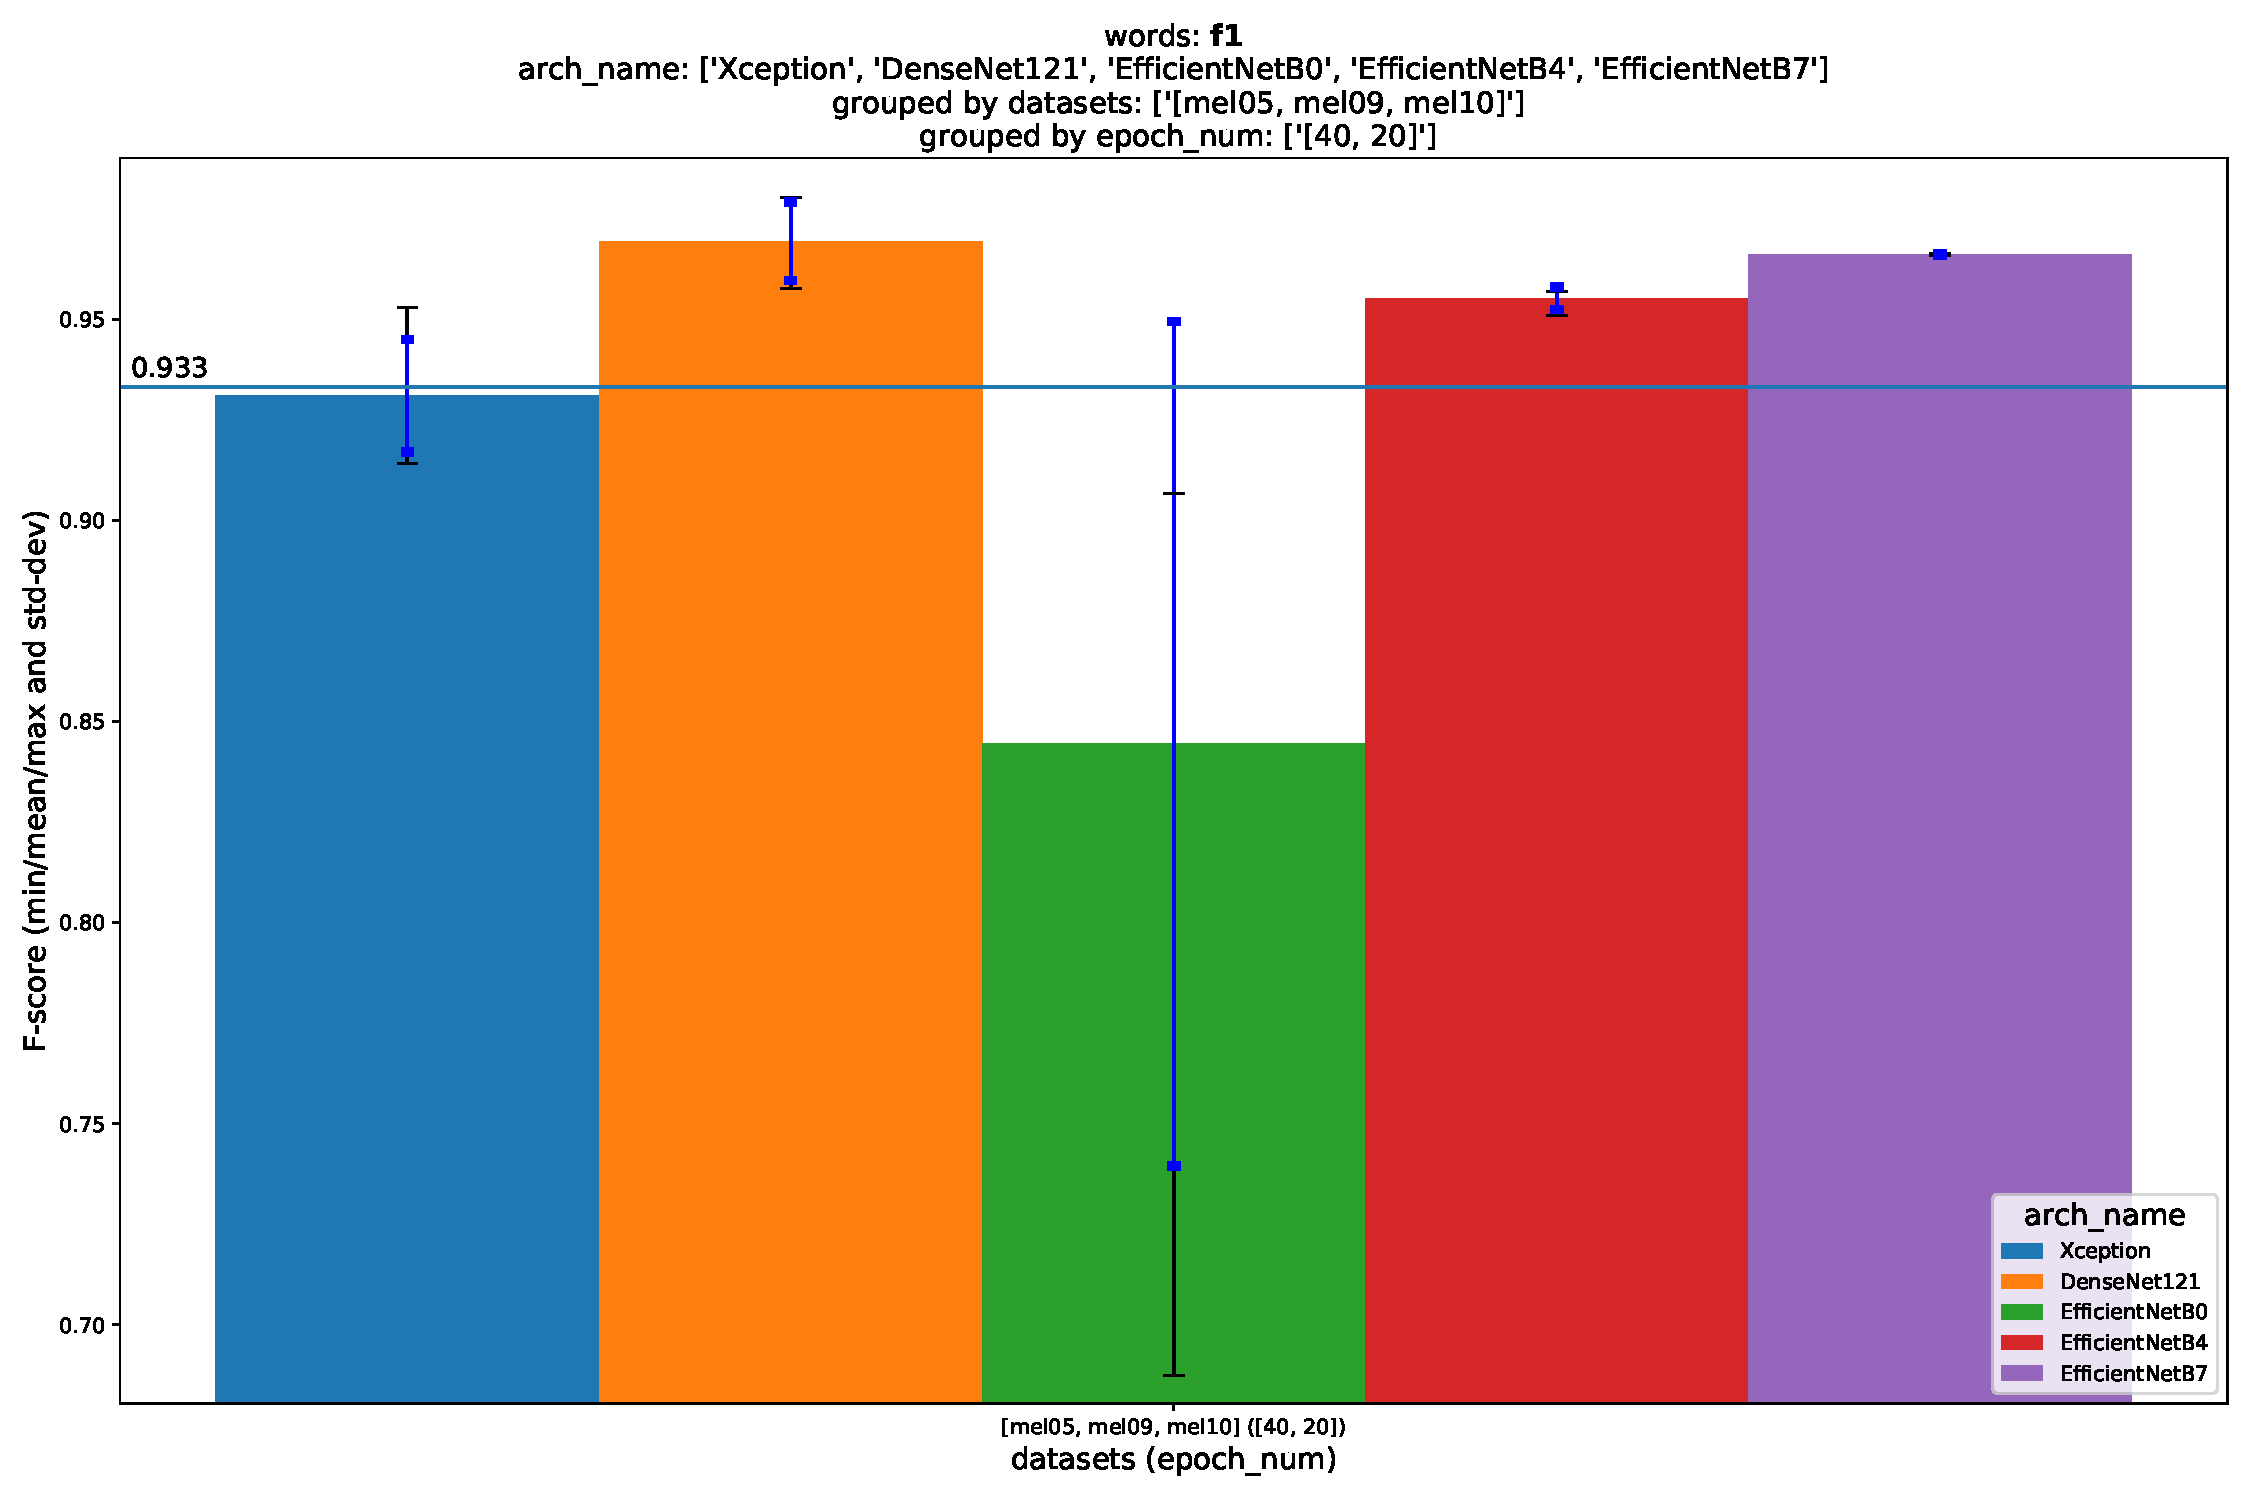
\includegraphics[width=0.8\linewidth]{Fscore_TRA_arch_comparison.pdf}
    \caption{Architecture TRA comparison}%
    \label{fig:tra_comparison_arch}
\end{figure}

\subsection{Hyper-parameter analysis: Attention}

A total of $1688$
% TODO
experiment were performed for the LSTM+attention model.

\subsubsection{Model parameters performance comparison}

\fig{fig:att_dropout_conv_query_dense} shows F-score values for 
variation of 
a)
the width of the dense classifier ($32$ or $64$),
b)
the dropout rate
after the initial convolutional layers
($0.2$ or $0$),
c)
the number of initial convolutional layers ($1$ or $2$)
and
d)
the query style ($01$ and $05$ pick a single LSTM vector to compute the scores,
$02$ and $03$ use convolutional layers connected to the LSTM outputs to extract
the scores and $04$  uses convolutional layers connected to the spectrograms).
The results are very close but two conclusions can be tentatively reached:

\begin{itemize}
    \item The query type does not influence the results: within each packet of
        columns the values are very close to each other, within one standard
        deviation.
    \item The combination of dense 02 ($64$ units), conv 01 ($1$ layer) and
        dropout 01 ($0.2$) seems to be consistently better than the average.
        The best values might be found with other combinations of parameters,
        but those combinations are less robust, as indicated by the higher
        standard deviation, and the quality of the model is less assured when
        training that combination for new datasets.
\end{itemize}

\begin{figure*}[t!]
    \centering
    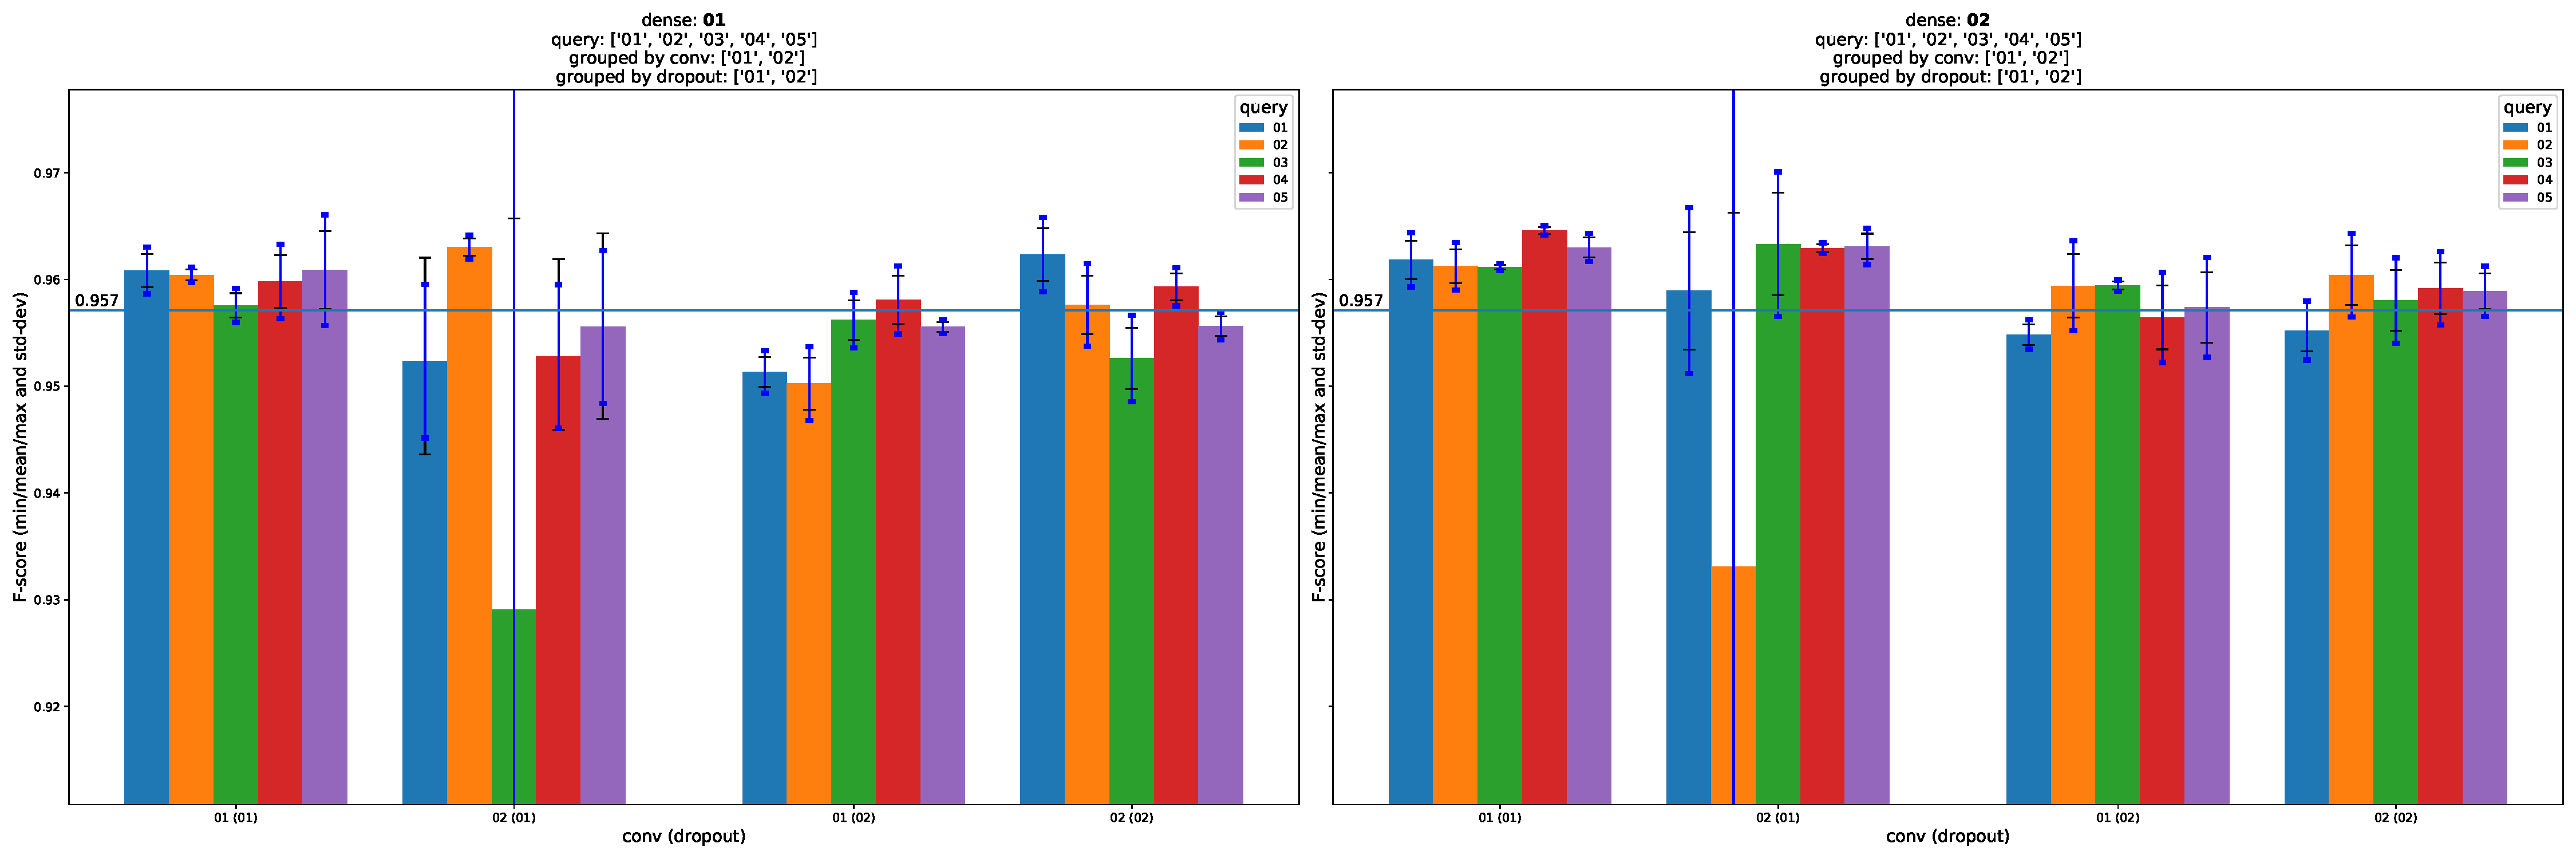
\includegraphics[width=0.9\linewidth]{Fscore_att2_dropout__conv__query__dense.pdf}
    \caption{F-score for varying
        dense classifier width,
        query type,
        convolution type,
        dropout.
        Averaged on 20 and 35 words task, solved by the LSTM+attention architecture.
        % MAYBE should also average on non ugmented dataset
        }%
    \label{fig:att_dropout_conv_query_dense}
\end{figure*}

\subsubsection{Training parameters performance comparison}

% Optimizer is fixed

\fig{fig:att_epoch_batch_lr_words} shows F-score values for 
variation of 
the number of training epochs ($2$, $4$, $15$ and $30$),
the batch size ($16$ or $32$),
and the learning rate
when the LSTM+attention model solves the task \texttt{k1}
on non-augmented datasets.
Two main conclusions can be reached:
\begin{itemize}
    \item
        The training gets more stable as the epoch number increases, and when
        using a larger batch size. For $30$ and $32$ respectively the results
        are quite consistent across the different learning rate types.
    \item
        The learning rate schedule \texttt{clr\_tri2\_04} (a cyclic learning
        rate with triangular 2 shape), when using enough epochs and a large
        batch size, is the one that performs the best.
\end{itemize}

\begin{figure*}[t!]
    \centering
    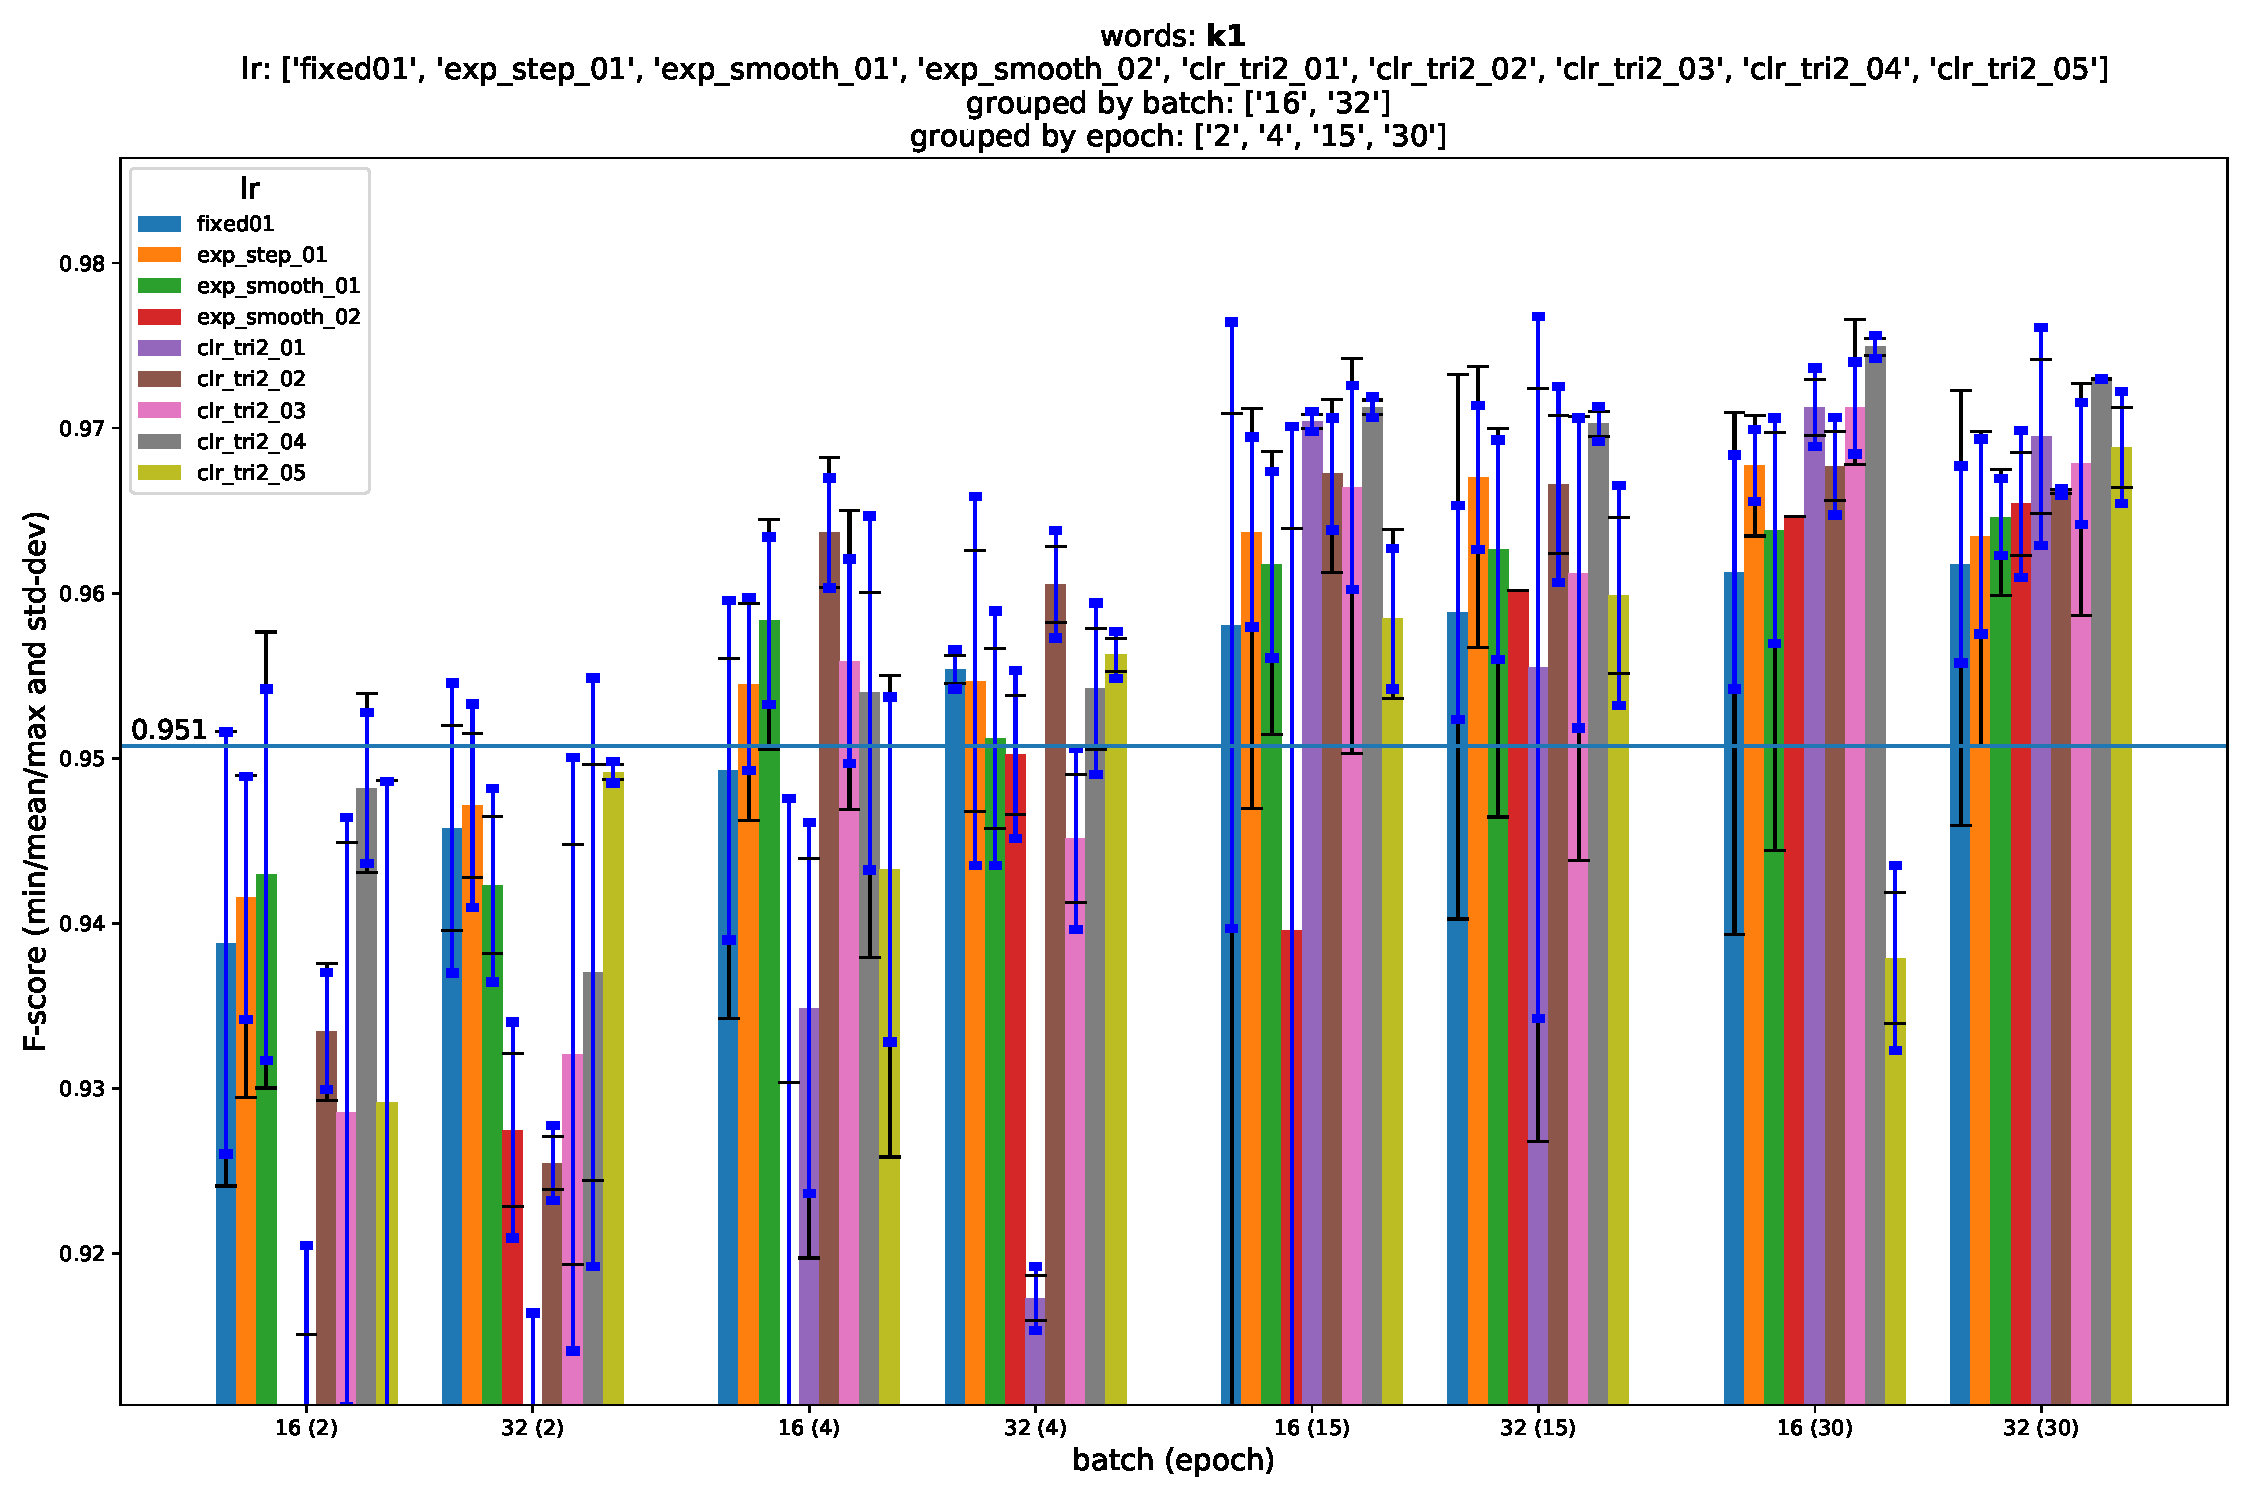
\includegraphics[width=0.9\linewidth]{Fscore_att2_epoch__batch__lr__words.pdf}
    \caption{F-score for varying
        epoch num,
        batch size,
        learning rate type,
        words type.
        Averaged on non-augmented datasets.
        Solved by the LSTM+attention architecture.
        }%
    \label{fig:att_epoch_batch_lr_words}
\end{figure*}

\subsection{AreaNet and SimpleNet performance}

TODO: So good!

\subsection{Data augmentation performance}
\label{sec:augmentation_performance}

% TODO: combine 01 and 15 for the final augmentation

As explained in \secref{sec:data_augmentation}, several types of augmentation
were performed on the dataset.
%
% MAYBE: type 01 aug was tested but too long The augmentation regarding the
% signal (i.e. \texttt{aug01}) was tested very little as it produced datasets
% that were too large to 
%
% The bulk of the investigation was to determine which kind of augmentation
% performed better.
Each type of augmentation is based on one set of spectrogram parameters, and
there are four styles of warp based aumentation: the landmarks are shifted 1)
along both axes of the spectrogram, 2) only along the time axis, 3) only along
the frequency axis, 4) along no axis, to provide a reference measure. Three
different spectrogram parameters and two different warping parameters were
tested. \tab{tab:aug_values}, in the Appendix, shows the specific values used.
For the ``big'' type, $3$ landmarks are shifted by at most $5$ units, while for
the ``small'' type, $4$ landmarks are shifted by at most $2$ units.
% The main differences in augmentation can be seen between the ``big'' and
% ``small'' types.
This leads to the largest difference in augmentation performance:
\tab{tab:augmentation_comparison_performance} shows that the ``small''
augmentation type leads to an increase in F-Score value of $0.015$ and $0.03$
relative to the ``big'' augmentation, when training the convolutional
architecture (\secref{sec:convolutional_arch}) on a 4-words task, and the
LSTM+attention model (\secref{sec:attention_model}) on a 10-words task
respectively.
%
This makes sense: the spectrograms used for augmentation have shape $(64, 64)$,
so moving a landmark by $5$ changes too sharply the image. A more uniform
augmentation, with more landmarks but with gentler warping leads to better
results.
%
For the convolutional architecture the mean F-Score value for the \texttt{f1}
4-words task increases from $0.939$ to $0.960$, while for the LSTM+attention
architecture, data augmentation does not increase the performance of the model.
However, the speed with which a high performance is achieved is influenced by
the presence of augmented data. As shown in
\tab{tab:augmentation_learning_speed} and in
\fig{fig:augmentation_learning_speed}, peak performance for the model is
reached after just $4$ epochs of training, compared to $10$ to $15$ epochs when
using non-augmented data.

\begin{table}[t!]
    \centering
    % \caption{Comparison between regular and augmented datasets:}
    \caption{Comparison between different types of augmentation,
    for the 10-words task solved by LSTM+attention architecture and a
    4-words task solved by the convolutional architecture.
    A reference non-augmented, well performing dataset is added.}
    \label{tab:augmentation_comparison_performance}
    \begin{tabular}{|cc|c|}
        \hline
        Aug ID & Spec+Type & F-Score \\
        \hline
        \hline
        % CNN & & (4 words)  \\
        % \multicolumn{2}{|c}{CNN} & (4 words) \\
        \multicolumn{3}{|c|}{CNN (4-words task)} \\
        % \hline
        % \hline
        % Aug ID & Spec+Type & F-Score \\
        \hline
        mel04 & None & $0.939 \pm 0.017$ \\
        02,03,04 & mel\_02+big   & $0.940 \pm 0.014$ \\
        06,07,08 & mel\_01+big   & $0.945 \pm 0.015$ \\
        10,11,12 & mel\_03+big   & $0.946 \pm 0.014$ \\
        14,15,16 & mel\_03+small & $0.960 \pm 0.008$ \\
        \hline
        \hline
        % \multicolumn{2}{c}{Multi-column}
        % LSTM+att & & (10 words) \\
        \multicolumn{3}{|c|}{LSTM+att (10-words task)} \\
        \hline
        % mel01   &  0.954 & 0.0073 \\
        mel04   &  None & $0.963 \pm 0.0126$ \\
        % mel05   & None &  $0.954 \pm 0.0184$ \\
        % mela1   &  0.958 & 0.0155 \\
        02,03,04 & mel\_02+big   &  $0.929 \pm 0.0362$ \\
        06,07,08 & mel\_01+big   &  $0.939 \pm 0.0392$ \\
        10,11,12 & mel\_03+big   &  $0.932 \pm 0.0852$ \\
        14,15,16 & mel\_03+small &  $0.964 \pm 0.0129$ \\
        \hline
    \end{tabular}
\end{table}

\begin{table}[t!]
    \centering
    \caption{Comparison of learning speed when training the LSTM+attention
    model on the $10$-words task \texttt{k1}.}
    \label{tab:augmentation_learning_speed}
    \begin{tabular}{|c|c|c|}
        \hline
        Epoch num & Regular & Augmented \\
        \hline
        2 & $0.923 \pm 0.034$ & $0.941 \pm 0.019$ \\
        4 & $0.948 \pm 0.016$ & $0.958 \pm 0.011$ \\
        15 & $0.959 \pm 0.013$ & $0.962 \pm 0.014$ \\
        \hline
    \end{tabular}
\end{table}

\begin{figure}[t!]
    \centering
    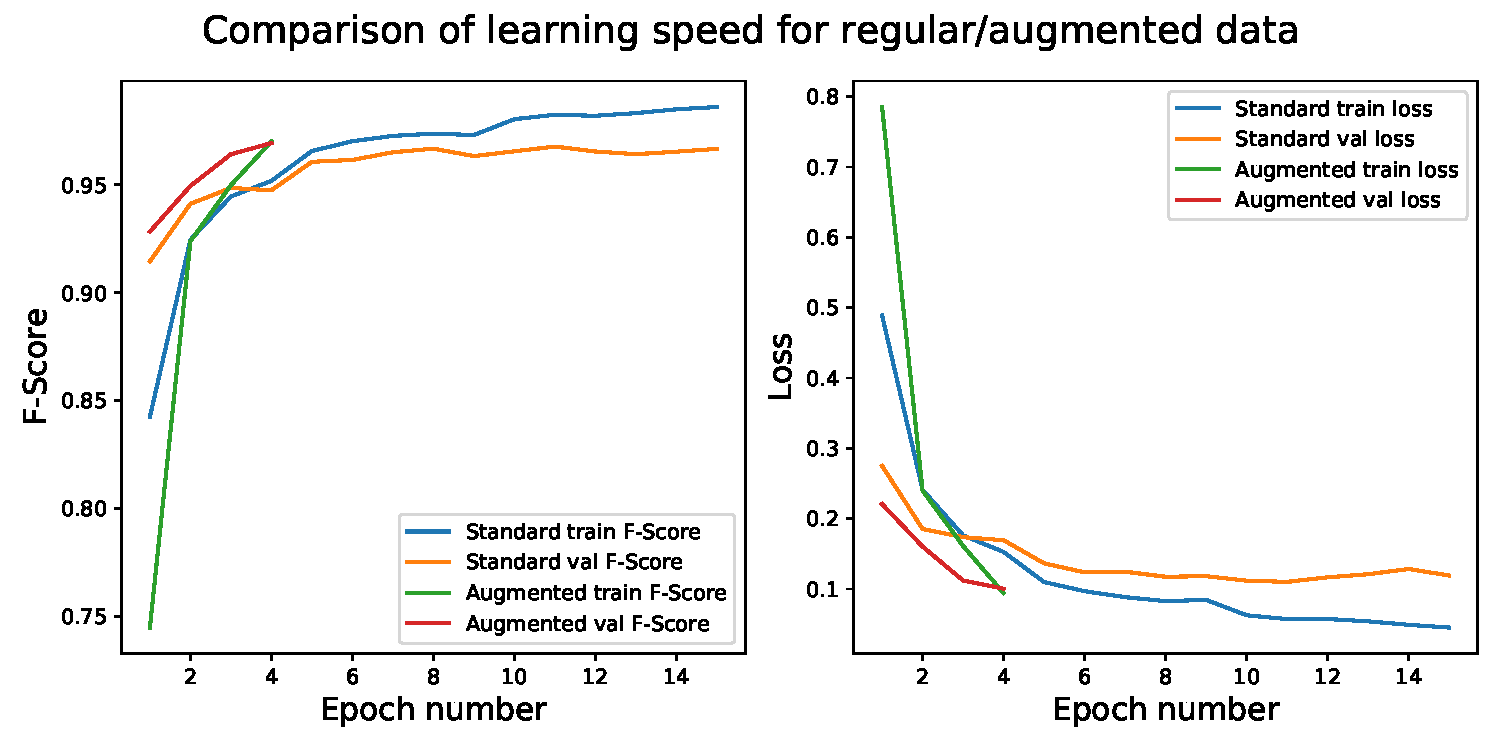
\includegraphics[width=0.9\linewidth]{comparison_augmentation.pdf}
    \caption{Comparison of the learning speed on regular vs. augmented data.}%
    \label{fig:augmentation_learning_speed}
\end{figure}

In \tab{tab:att_augmentation_comparison} the different types of
augmentation, along different axis, are compared:
no particular type emerges as better than the others.

\begin{table}[t!]
    \centering
    \caption{Comparison between different styles of augmentation,
    for the 10-words task solved by LSTM+attention architecture and a
    4-words task solved by the convolutional architecture.}
    \label{tab:att_augmentation_comparison}
    \begin{tabular}{|c|c|}
        \hline
        Augmentation type & F-Score \\
        \hline
        \hline
        \multicolumn{2}{|c|}{LSTM+attention (10 words task)} \\
        \hline
        Both axis & $0.9326 \pm 0.0615$ \\
        Time      & $0.9448 \pm 0.0323$ \\
        Frequency & $0.9355 \pm 0.0383$ \\
        None      & $0.9311 \pm 0.0794$ \\
        \hline
        \hline
        \multicolumn{2}{|c|}{CNN (4 words task)} \\
        \hline
        Both axis & $0.945 \pm 0.016$ \\
        Time      & $0.946 \pm 0.014$ \\
        Frequency & $0.944 \pm 0.014$ \\
        None      & $0.940 \pm 0.016$ \\
        \hline
    \end{tabular}
\end{table}

%%%%%%%%%%%%%%%%%%%

\subsection{Extract loudest section performance}

As an additional preprocessing step, the loudest $0.5$s section of the audio
signal was selected.
%
It might seem surprising, but both the LSTM+attention and the AreaNet
architectures performed better on the full audio samples, 
as shown in \tab{tab:comparison_loud_section}.
%
This however could partly be explained by the fact that those are \textit{attention}
architectures, so by design they will identify the relevant portion of the data.
By only feeding important data to the networks, the attention mechanism has more
difficulty to learn which sections to select, because all of them are useful.
%
On the other hand, the SimpleNet was also trained on the loudest section of the data
and that also did not lead to an improvement.
% MAYBE

\begin{table}[t!]
    \centering
    \caption{Comparison of the original dataset and the dataset that only
    includes the loudest section of the audio samples.}
    \label{tab:comparison_loud_section}
    \begin{tabular}{|c|c|c|}
        \hline
        & LTnum & LTnumLS \\
        \hline
        CNN      & $0.967 \pm 0.000$ & $0.952 \pm 0.003$ \\
        LSTM+att & $0.969 \pm 0.012$ & $0.953 \pm 0.012$ \\
        AreaNet  & $0.977 \pm 0.011$ & $0.962 \pm 0.023$ \\
        \hline
        % & LSTM+att & AreaNet(s) \\
        % LTnum   & $0.969 \pm 0.012$ & $0.977 \pm 0.011$ \\
        % LTnumLS & $0.953 \pm 0.012$ & $0.962 \pm 0.023$ \\
    \end{tabular}
\end{table}

\subsection{Architecture comparison}

\subsubsection{F-Score performance}

\tab{tab:mega_comparison} shows the results for all architectures and tasks,
listing the F-Score mean, standard deviation and max values.
%
The best performances are achieved by the SimpleNet in its larger variant. This
architecture performs well not only regarding to the best model in the class,
but also according to the very low standard deviation values, that indicate a
very robust training.
%
The VerticalAreaNet tends to perform better than the AreaNet, showing that
emphasizing the temporal correlations helps the training as the attention
weights only have to select the relevant \textit{temporal} portion of the
input, while selecting also along the frequency axes (as AreaNet does) does not
improve performances.
%
It is expected that on a standard image dataset, that lacks this vertical
correlation, AreaNet would perform better than VerticalAreaNet.

% % Autogenerated by python evaluate_all.py -et build_megacomparison_v03
% Mildly modified
\begin{table*}[t!]
    \centering
    \caption{Architecture comparison for different tasks. Each cell shows the mean, standard deviation and max F-Score value.}
    \label{tab:mega_comparison}
    \begin{tabular}{|c|ccccc|}
        \hline
        Arch & f1 & k1 & yn & num, LTnum, LTBnum & all, LTall, LTBall \\
        \hline
        \hline
        \multirow{2}{*}{CNN}
             & $0.918 \pm 0.037$ & -                 & -                 & $0.955 \pm 0.010$ & $0.879 \pm 0.040$ \\
             & $    0.980 $      & -                 & -                 & $    0.970 $      & $    0.909 $      \\
        \hline
        \multirow{2}{*}{TRA}
             & $0.878 \pm 0.091$ & -                 & $0.977 \pm 0.002$ & $0.945 \pm 0.009$ & -                 \\
             & $    0.953 $      & -                 & $    0.978 $      & $    0.951 $      & -                 \\
        \cline{2-6}
        \multirow{2}{*}{TD1}
             & $0.960 \pm 0.024$ & $0.959 \pm 0.008$ & $0.988 \pm 0.003$ & $0.970 \pm 0.008$ & $0.948 \pm 0.003$ \\
             & $    0.980 $      & $    0.964 $      & $    0.990 $      & $    0.977 $      & $    0.950 $      \\
        \cline{2-6}
        \multirow{2}{*}{TB0}
             & $0.844 \pm 0.105$ & $0.898 \pm 0.035$ & -                 & $0.938 \pm 0.016$ & $0.902 \pm 0.001$ \\
             & $    0.907 $      & $    0.919 $      & -                 & $    0.946 $      & $    0.903 $      \\
        \cline{2-6}
        \multirow{2}{*}{TB4}
             & $0.955 \pm 0.003$ & -                 & $0.994 \pm 0.000$ & $0.954 \pm 0.003$ & $0.910 \pm 0.002$ \\
             & $    0.957 $      & -                 & $    0.994 $      & $    0.958 $      & $    0.911 $      \\
        \cline{2-6}
        \multirow{2}{*}{TB7}
             & $0.966 \pm 0.000$ & -                 & -                 & -                 & -                 \\
             & $    0.966 $      & -                 & -                 & -                 & -                 \\
        \hline
        \multirow{2}{*}{ATT}
             & $0.962 \pm 0.011$ & $0.946 \pm 0.033$ & $0.988 \pm 0.010$ & $0.969 \pm 0.012$ & $0.948 \pm 0.003$ \\
             & $    0.978 $      & $    0.977 $      & $    0.996 $      & $    0.978 $      & $    0.952 $      \\
        \hline
        \multirow{2}{*}{SIM}
             & $0.982 \pm 0.005$ & $0.975 \pm 0.002$ & $0.995 \pm 0.004$ & $0.981 \pm 0.003$ & $0.953 \pm 0.006$ \\
             & $    0.989 $      & $    0.978 $      & $\bf{0.999}$      & $    0.986 $      & $    0.960 $      \\
        \cline{2-6}
        \multirow{2}{*}{SI2}
             & $0.984 \pm 0.004$ & $0.978 \pm 0.003$ & $0.997 \pm 0.002$ & $0.984 \pm 0.003$ & $0.963 \pm 0.002$ \\
             & $\bf{0.990}$      & $\bf{0.982}$      & $\bf{0.999}$      & $\bf{0.988}$      & $\bf{0.967}$      \\
        \cline{2-6}
        \multirow{2}{*}{AAN}
             & $0.947 \pm 0.028$ & $0.879 \pm 0.102$ & $0.940 \pm 0.113$ & $0.971 \pm 0.020$ & $0.948 \pm 0.010$ \\
             & $    0.979 $      & $    0.954 $      & $    0.996 $      & $    0.985 $      & $    0.962 $      \\
        \cline{2-6}
        \multirow{2}{*}{VAN}
             & $0.964 \pm 0.018$ & $0.969 \pm 0.005$ & $0.950 \pm 0.094$ & $0.975 \pm 0.011$ & $0.948 \pm 0.013$ \\
             & $    0.979 $      & $    0.978 $      & $\bf{0.999}$      & $    0.986 $      & $    0.961 $      \\
        \hline
    \end{tabular}
\end{table*}


% Autogenerated by python evaluate_all.py -et evaluate_results_all
\begin{table*}[t!]
    \centering
    \caption{Mega comparison}
    \label{tab:mega_comparison}
    \begin{tabular}{|c|ccc|}
        \hline
        \multicolumn{4}{|c|}{Task: f1} \\
        \hline
        Arch & Mean $\pm$ StdDev & Min & Max \\
        \hline
        CNN & $0.832 \pm 0.109$ & $0.501$ & $0.978$ \\
        TRA & $0.868 \pm 0.099$ & $0.521$ & $0.953$ \\
        TD1 & $0.960 \pm 0.024$ & $0.920$ & $0.980$ \\
        TB0 & $0.844 \pm 0.105$ & $0.687$ & $0.907$ \\
        TB4 & $0.955 \pm 0.003$ & $0.951$ & $0.957$ \\
        TB7 & $0.966 \pm 0.000$ & $0.966$ & $0.966$ \\
        ARN & $0.979 \pm 0.011$ & $0.960$ & $\bf{0.986}$ \\
        \hline
        \hline
        \multicolumn{4}{|c|}{Task: k1} \\
        \hline
        Arch & Mean $\pm$ StdDev & Min & Max \\
        \hline
        TD1 & $0.959 \pm 0.008$ & $0.950$ & $0.964$ \\
        TB0 & $0.898 \pm 0.035$ & $0.847$ & $0.919$ \\
        ATT & $0.946 \pm 0.031$ & $0.729$ & $\bf{0.977}$ \\
        \hline
        \hline
        \multicolumn{4}{|c|}{Tasks: yn, LTyn} \\
        \hline
        Arch & Mean $\pm$ StdDev & Min & Max \\
        \hline
        AAN & $0.941 \pm 0.131$ & $0.529$ & $0.990$ \\
        ARN & $0.997 \pm 0.003$ & $0.995$ & $\bf{0.999}$ \\
        SIM & $0.992 \pm 0.003$ & $0.987$ & $0.998$ \\
        VAN & $0.991 \pm 0.004$ & $0.986$ & $0.998$ \\
        \hline
        \hline
        \multicolumn{4}{|c|}{Tasks: num, LTnum} \\
        \hline
        Arch & Mean $\pm$ StdDev & Min & Max \\
        \hline
        CNN & $0.954 \pm 0.012$ & $0.828$ & $0.970$ \\
        TRA & $0.945 \pm 0.009$ & $0.939$ & $0.951$ \\
        TD1 & $0.970 \pm 0.008$ & $0.960$ & $0.977$ \\
        TB0 & $0.938 \pm 0.016$ & $0.914$ & $0.946$ \\
        TB4 & $0.954 \pm 0.003$ & $0.951$ & $0.958$ \\
        ATT & $0.969 \pm 0.012$ & $0.911$ & $0.978$ \\
        AAN & $0.962 \pm 0.025$ & $0.917$ & $0.985$ \\
        ARN & $0.981 \pm 0.002$ & $0.978$ & $0.983$ \\
        SIM & $0.981 \pm 0.003$ & $0.975$ & $0.985$ \\
        SI2 & $0.981 \pm 0.004$ & $0.975$ & $\bf{0.986}$ \\
        VAN & $0.975 \pm 0.006$ & $0.964$ & $0.981$ \\
        \hline
        \hline
        \multicolumn{4}{|c|}{Tasks: all, LTall} \\
        \hline
        Arch & Mean $\pm$ StdDev & Min & Max \\
        \hline
        CNN & $0.863 \pm 0.057$ & $0.653$ & $0.901$ \\
        TD1 & $0.948 \pm 0.003$ & $0.946$ & $0.950$ \\
        TB0 & $0.902 \pm 0.001$ & $0.901$ & $0.903$ \\
        TB4 & $0.910 \pm 0.002$ & $0.908$ & $0.911$ \\
        ATT & $0.949 \pm 0.003$ & $0.946$ & $0.952$ \\
        AAN & $0.948 \pm 0.010$ & $0.927$ & $0.957$ \\
        ARN & $0.952 \pm 0.005$ & $0.944$ & $0.957$ \\
        SIM & $0.954 \pm 0.004$ & $0.948$ & $0.960$ \\
        SI2 & $0.963 \pm 0.001$ & $0.960$ & $\bf{0.965}$ \\
        VAN & $0.953 \pm 0.009$ & $0.932$ & $0.961$ \\
        \hline
    \end{tabular}
\end{table*}

Confusion matrices for VerticalAreaNet solving the ``yes/no'', ``LTBnum'' and
``LTBall'' tasks are shown in \fig{fig:VAN_opa1_lr03_bs32_en14_dsaug14_wyn_cm},
\fig{fig:VAN_opa1_lr03_bs32_en15_dsaug14_wLTBnum_cm} and
\fig{fig:VAN_opa1_lr03_bs32_en15_dsmel04_wLTBall_noval_cm} respectively.
%
\fig{fig:SI2_opa1_lr04_bs32_en15_dsmel04_wLTBall_noval_cm} shows the confusion
matrix for SimpleNet2 solving the ``LTBall'' task.
%
\fig{fig:ATT_ct02_dr01_ks01_lu01_qt01_dw01_opa1_lr03_bs02_en02_dsmel04_wLTBall_cm}
shows the confusion matrix for LSTM+attention model solving the ``LTBall''
task.

% TODO: visual wow
Note that for all architectures the largest mistake is regarding
the classification of ``wow'' that is sometimes predicted as ``visual''.
Indeed, the two words sound very similar: one of the possible pronunciations
for visual includes the 
% https://tex.stackexchange.com/a/370073
% /waʊ̯/
% 
\includegraphics[width=1em]{usound.pdf}
/
\includegraphics[width=0.6em]{usound.pdf}/
sound,
which is the main phoneme uttered when saying wow.

% TODO: 93.9% (35-word)


\begin{figure}[t!]
    \centering
    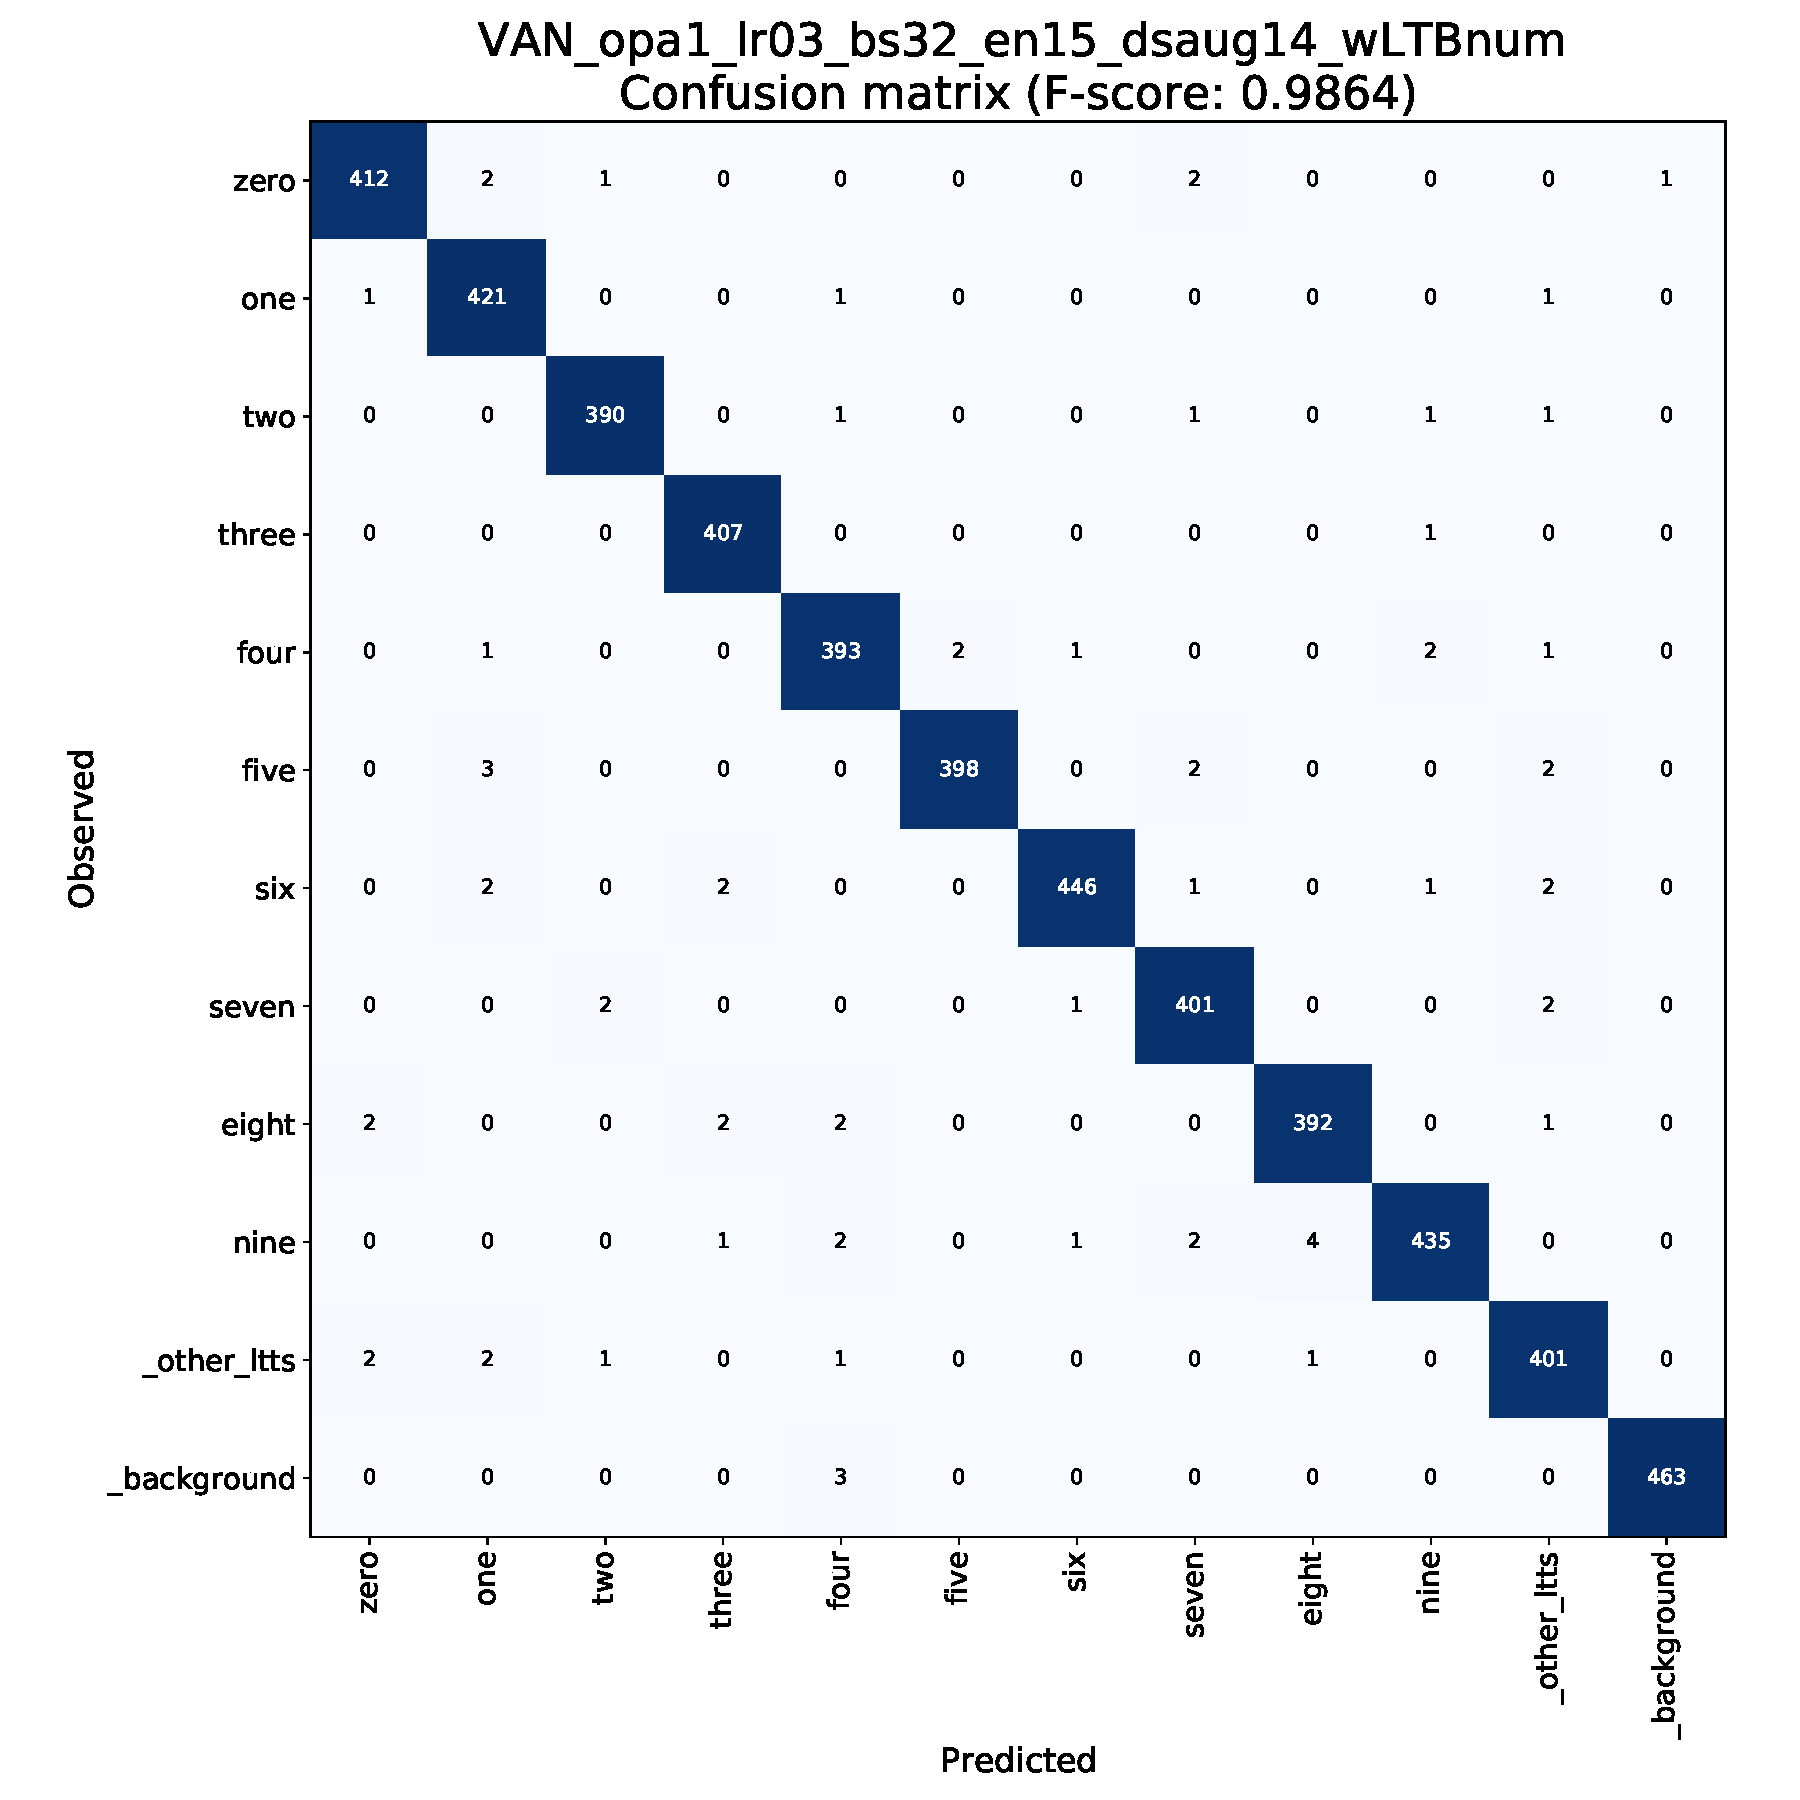
\includegraphics[width=0.9\linewidth]{VAN_opa1_lr03_bs32_en15_dsaug14_wLTBnum_cm.pdf}
    \caption{VAN opa1 lr03 bs32 en15 dsaug14 wLTBnum cm}%
    \label{fig:VAN_opa1_lr03_bs32_en15_dsaug14_wLTBnum_cm}
\end{figure}

\subsubsection{FSDD performance}

TODO: Test all on that, MAYBE merge with architecture comparision

\subsection{Attention weights}

% \subsubsection{Attention model}

% Show attention weights for Att model

The LSTM+attention model described in \secref{sec:attention_model} computes a query
vector that is used to weigh the LSTM outputs. Showing the attention weights
can help understand which parts of the recording were relevant for the
classification.
\fig{fig:attention_weights_standard} shows the spectrograms, the attention
weigths and the predictions for three sample words.
Indeed, the attention weights show which some sections of the data is more important
and is used to extract information from the signal.

% ATT_ct02_dr01_ks01_lu01_qt05_dw01_opa1_lr03_bs02_en02_dsaug07_wLTnum_LTnum_train_data
\begin{figure*}[t!]
    \centering
    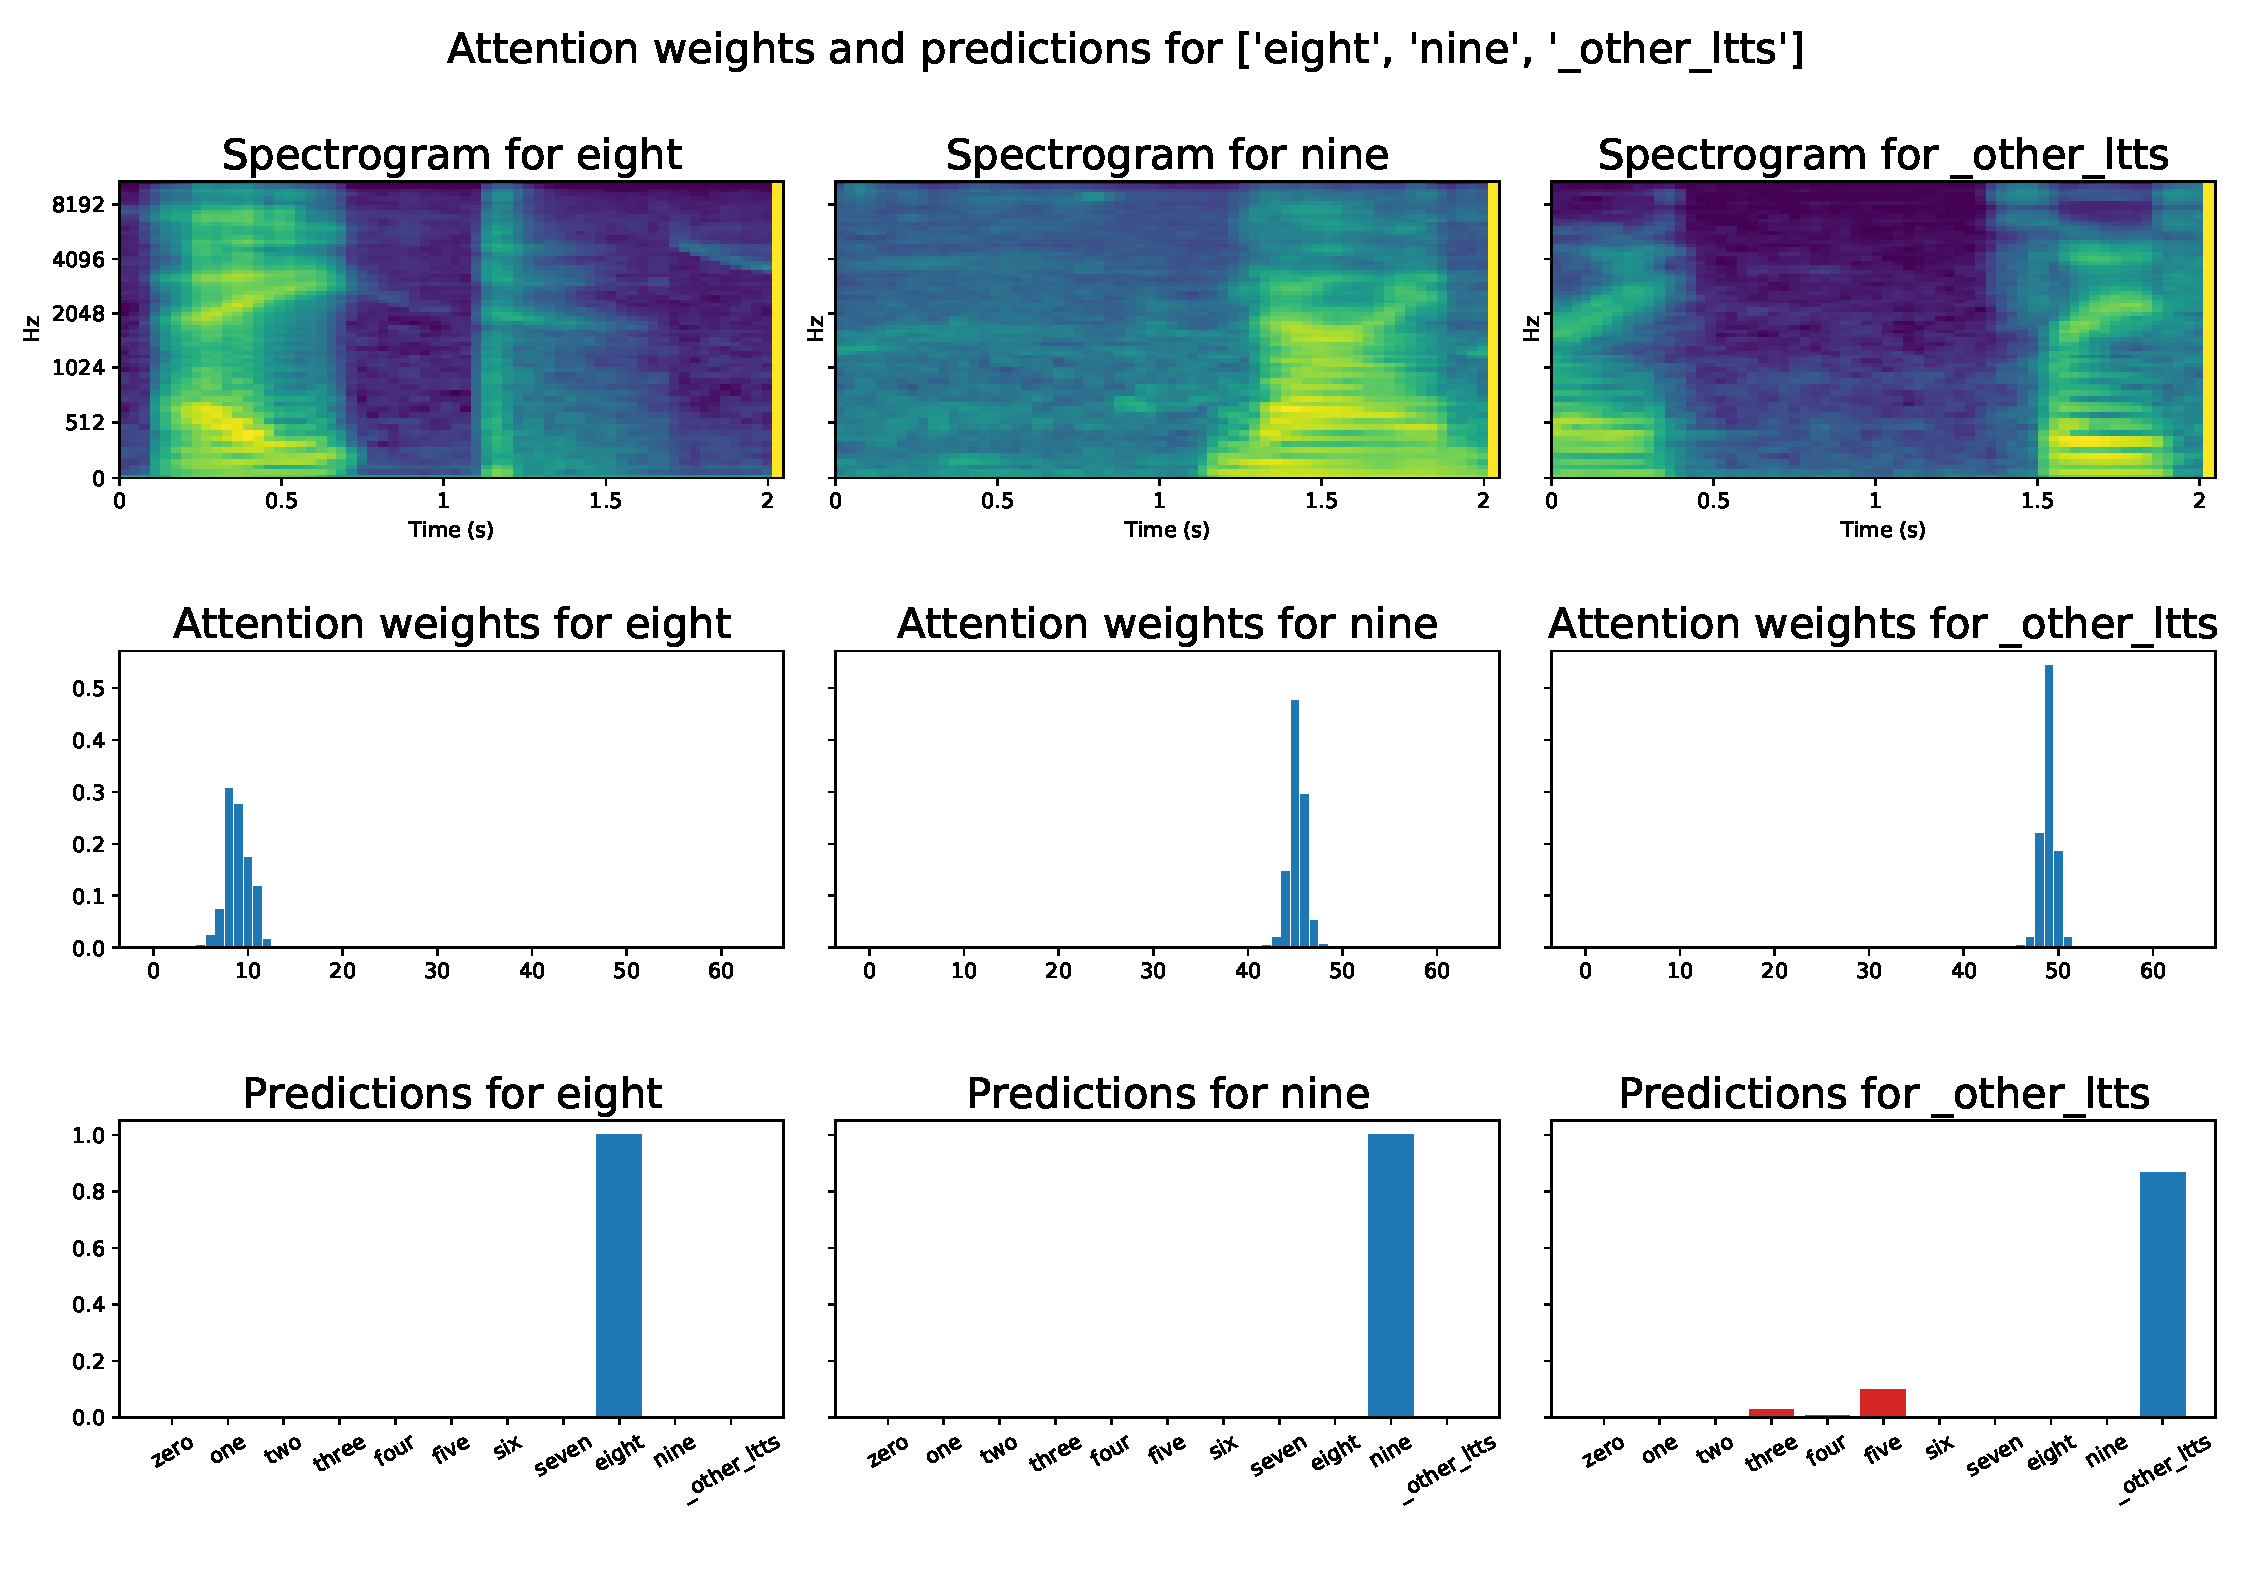
\includegraphics[width=0.9\linewidth]{ATT_ct02_dr01_ks01_lu01_qt05_dw01_opa1_lr03_bs02_en02_dsaug07_wLTnum_LTnum_train_data.pdf}
    \caption{Spectrograms, attention weights and predictions for three sample words.
    Notice how the attention weights correctly selected the interesting part of
    the ``eight'' spectrogram, avoiding the noise in the latter part.
    For ``\_other\_ltts'', which corresponds to a random audio snippet from the LibriTTS
    dataset, the attention weights still selected the section where a word is spoken,
    and, with some small uncertainty, the word is indeed recognized as ``other''.}%
    \label{fig:attention_weights_standard}
\end{figure*}

An example of the weights computed by AreaNet and VerticalAreaNet were already shown 
in \fig{fig:attention_weights_area} and \fig{fig:attention_weights_vertical}.

\subsection{Stream predictions}

The effectiveness of using a model trained on single word utterances to
identify a word in a sentence is examined in this section.
\fig{fig:stream_attention_ltts_meL04_LTnumLS_26} is an example of a very good
scenario: of the four numbers spoken, three are well isolated in the sentence,
and are clearly picked up. The initial utterance of ``three'' is also
identified, albeit with a lower probability, as it is very close to the next
word (``\textit{three} o'clock'' is spoken with barely a pause).
\fig{fig:stream_attention_ltts_meL04_LTnumLS_67} shows a more common situation,
when the interesting word is in the middle of the sentence (``of the
\textit{four} other\ldots''). The model can only barely identify the presence
of the word.
\fig{fig:stream_attention_ltts_meL04_LTnumLS_19} shows why a ``silence'' class
would be useful: when background converation is present, the model consistently
identifies \texttt{\_other} as the predicted word, but in the section where no
word is spoken, the model fires randomly.

Training only on the loudest $0.5$ second section of the audio samples improves
the performance of the models quite a lot: the ``four'' in the second example
is completely missed by a model trained with identical parameters except the
longer words, as shown in \fig{fig:stream_attention_ltts_mel04_LTnum_67}: only
the more isolated ``two'' is found, as there is space to align a window that
ends with the utterance and starts with silence.

A manual inspection was conducted on $116$ sentences containing numbers, and
only $31$ were correctly identified, amounting to $26.7\%$ recall.
The false positives however are only $14$, resulting in a precision of
$87.9\%$: if a number is identified, there is reasonable confidence that was
actually spoken.
% good_count: 31
% bad_count: 85
% total: 116

TODO: write meaningful captions

\begin{figure}[h!]
    \centering
    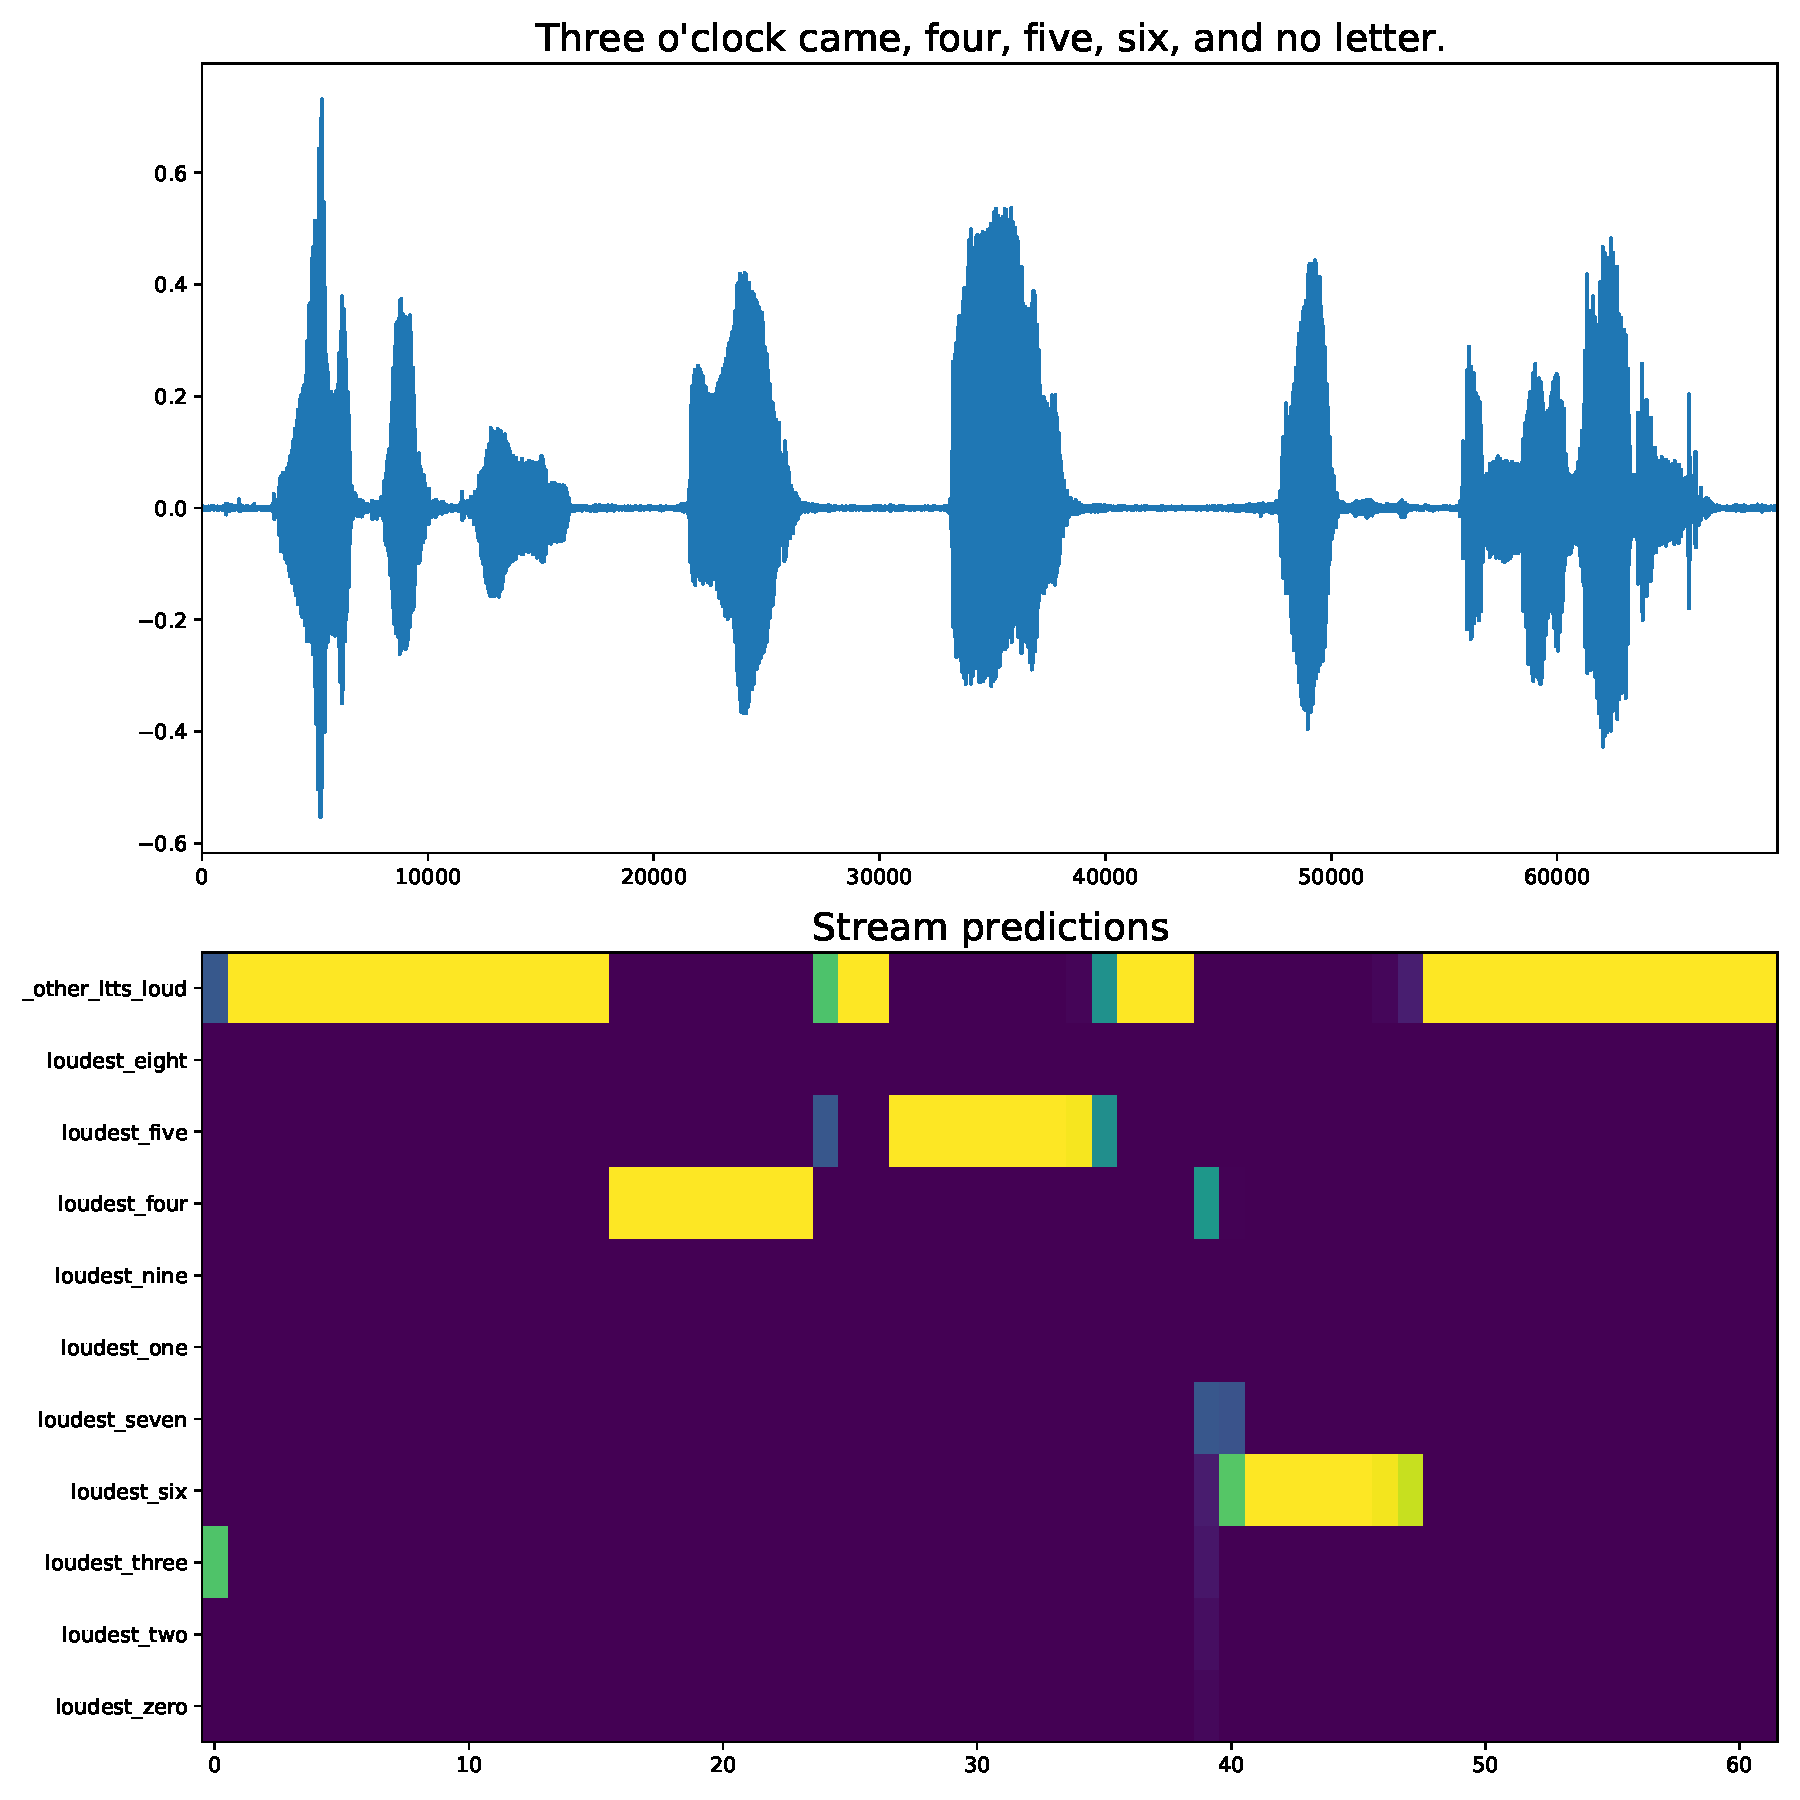
\includegraphics[width=0.9\linewidth]{stream2_attention_ltts_meL04_LTnumLS_26.pdf}
    \caption{Stream 26}%
    \label{fig:stream_attention_ltts_meL04_LTnumLS_26}
\end{figure}

\begin{figure}[h!]
    \centering
    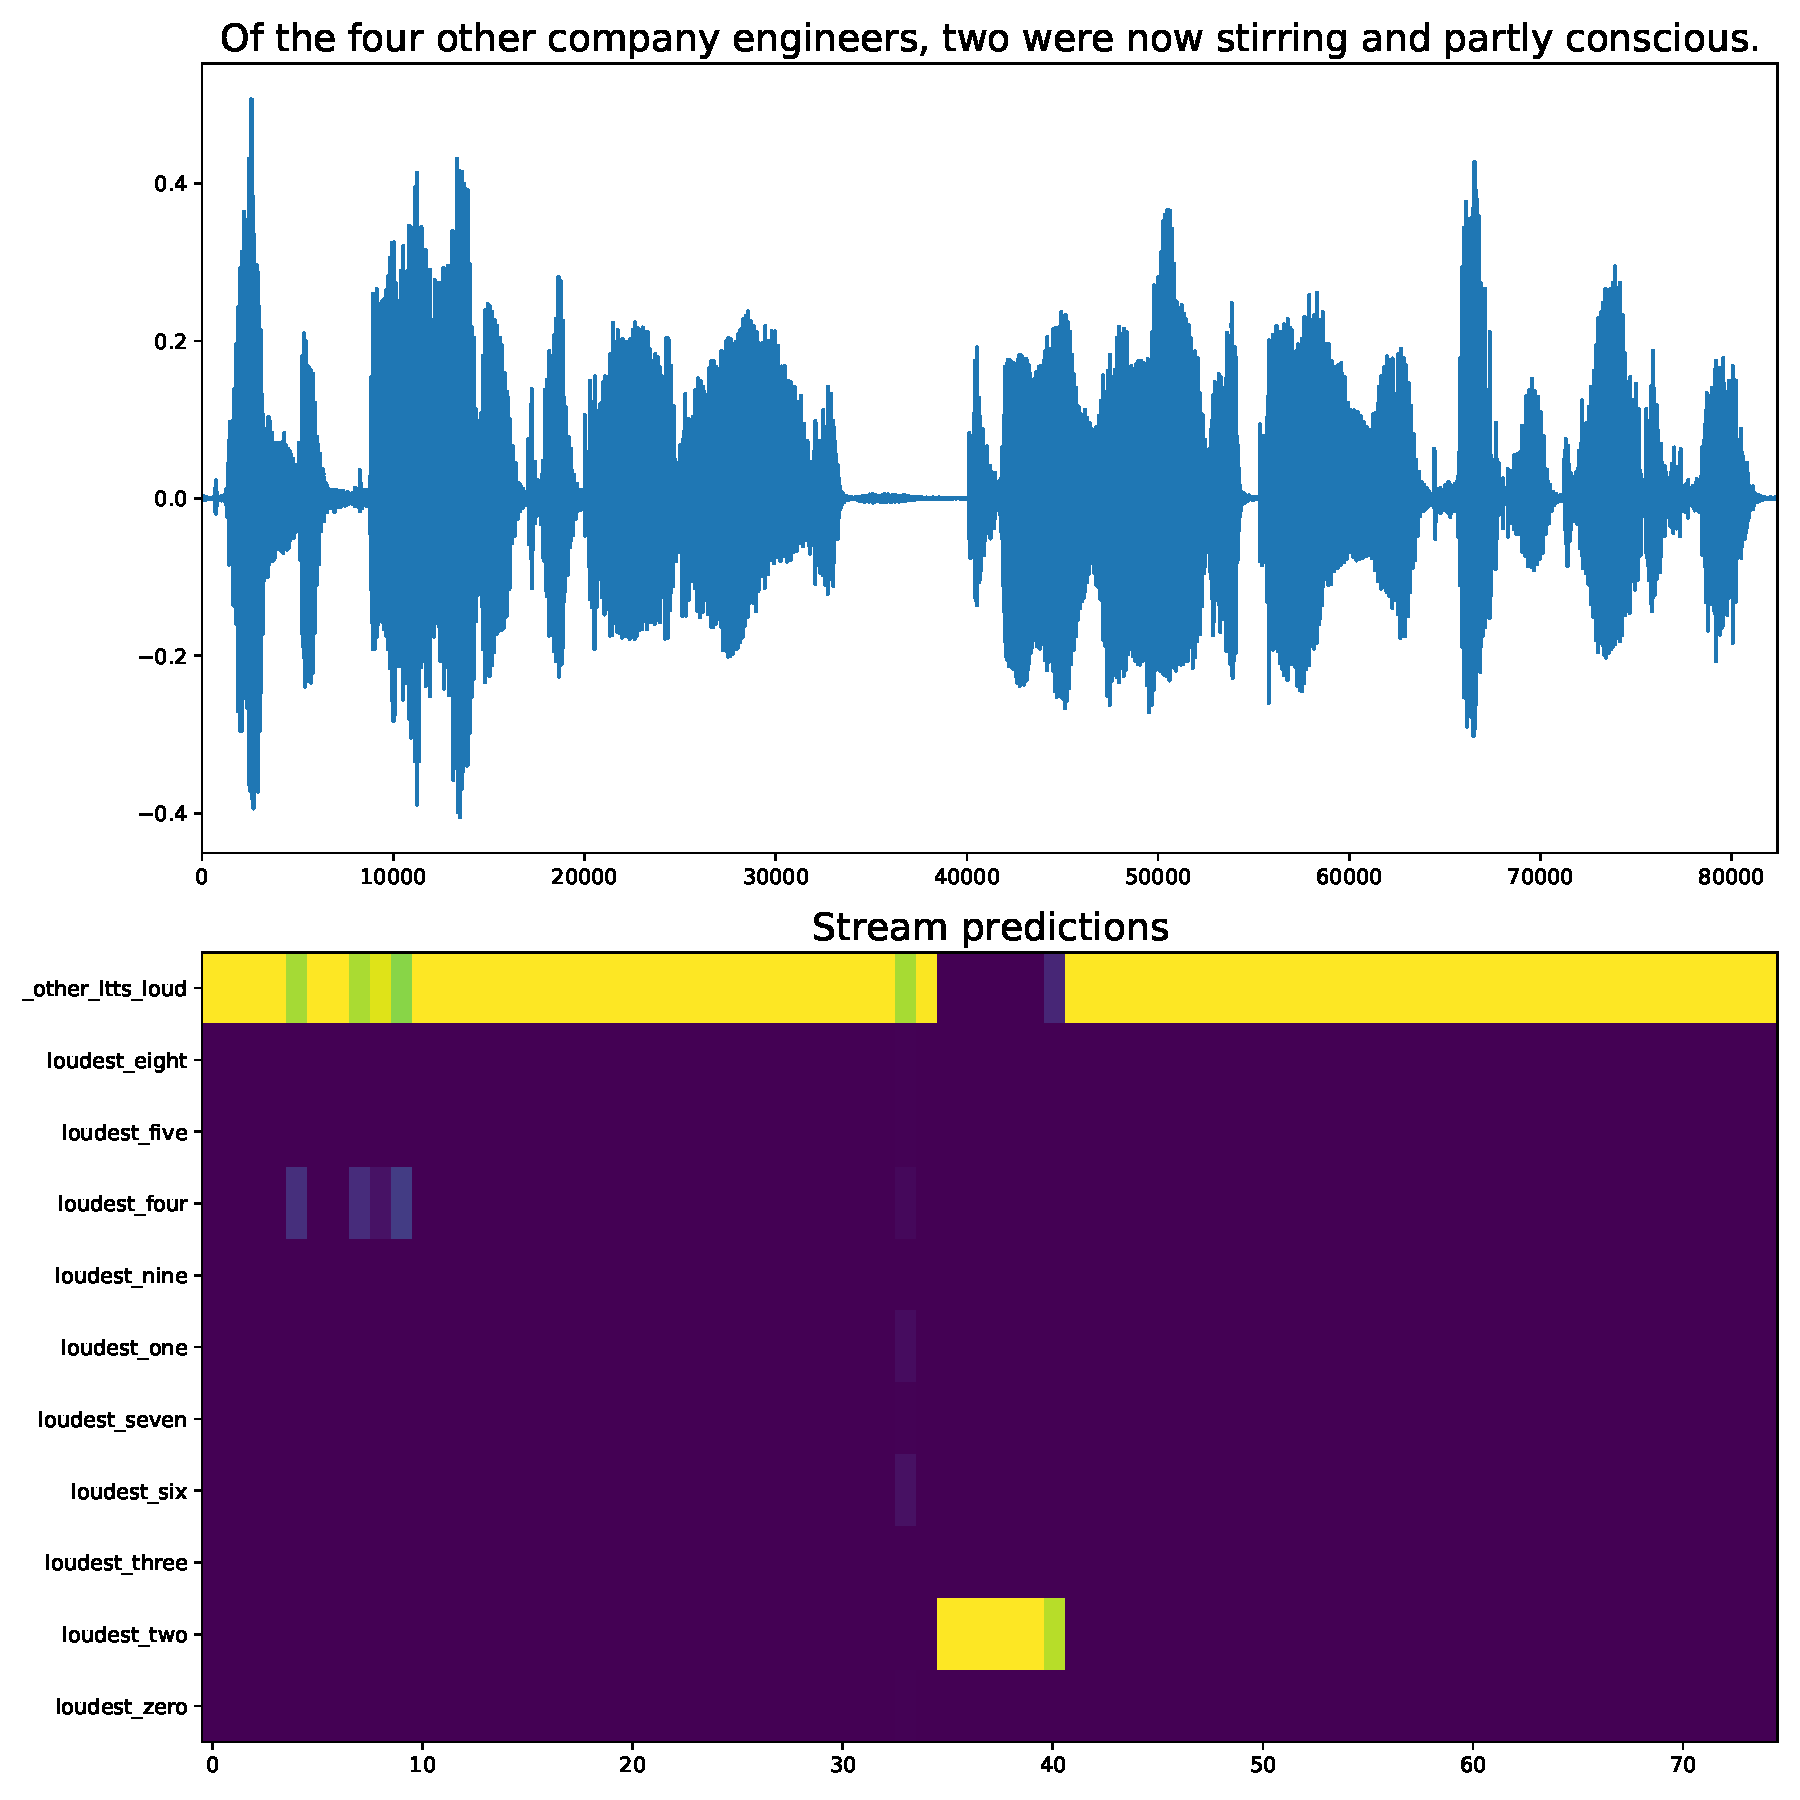
\includegraphics[width=0.9\linewidth]{stream2_attention_ltts_meL04_LTnumLS_67.pdf}
    \caption{Stream 67}%
    \label{fig:stream_attention_ltts_meL04_LTnumLS_67}
\end{figure}

\begin{figure}[h!]
    \centering
    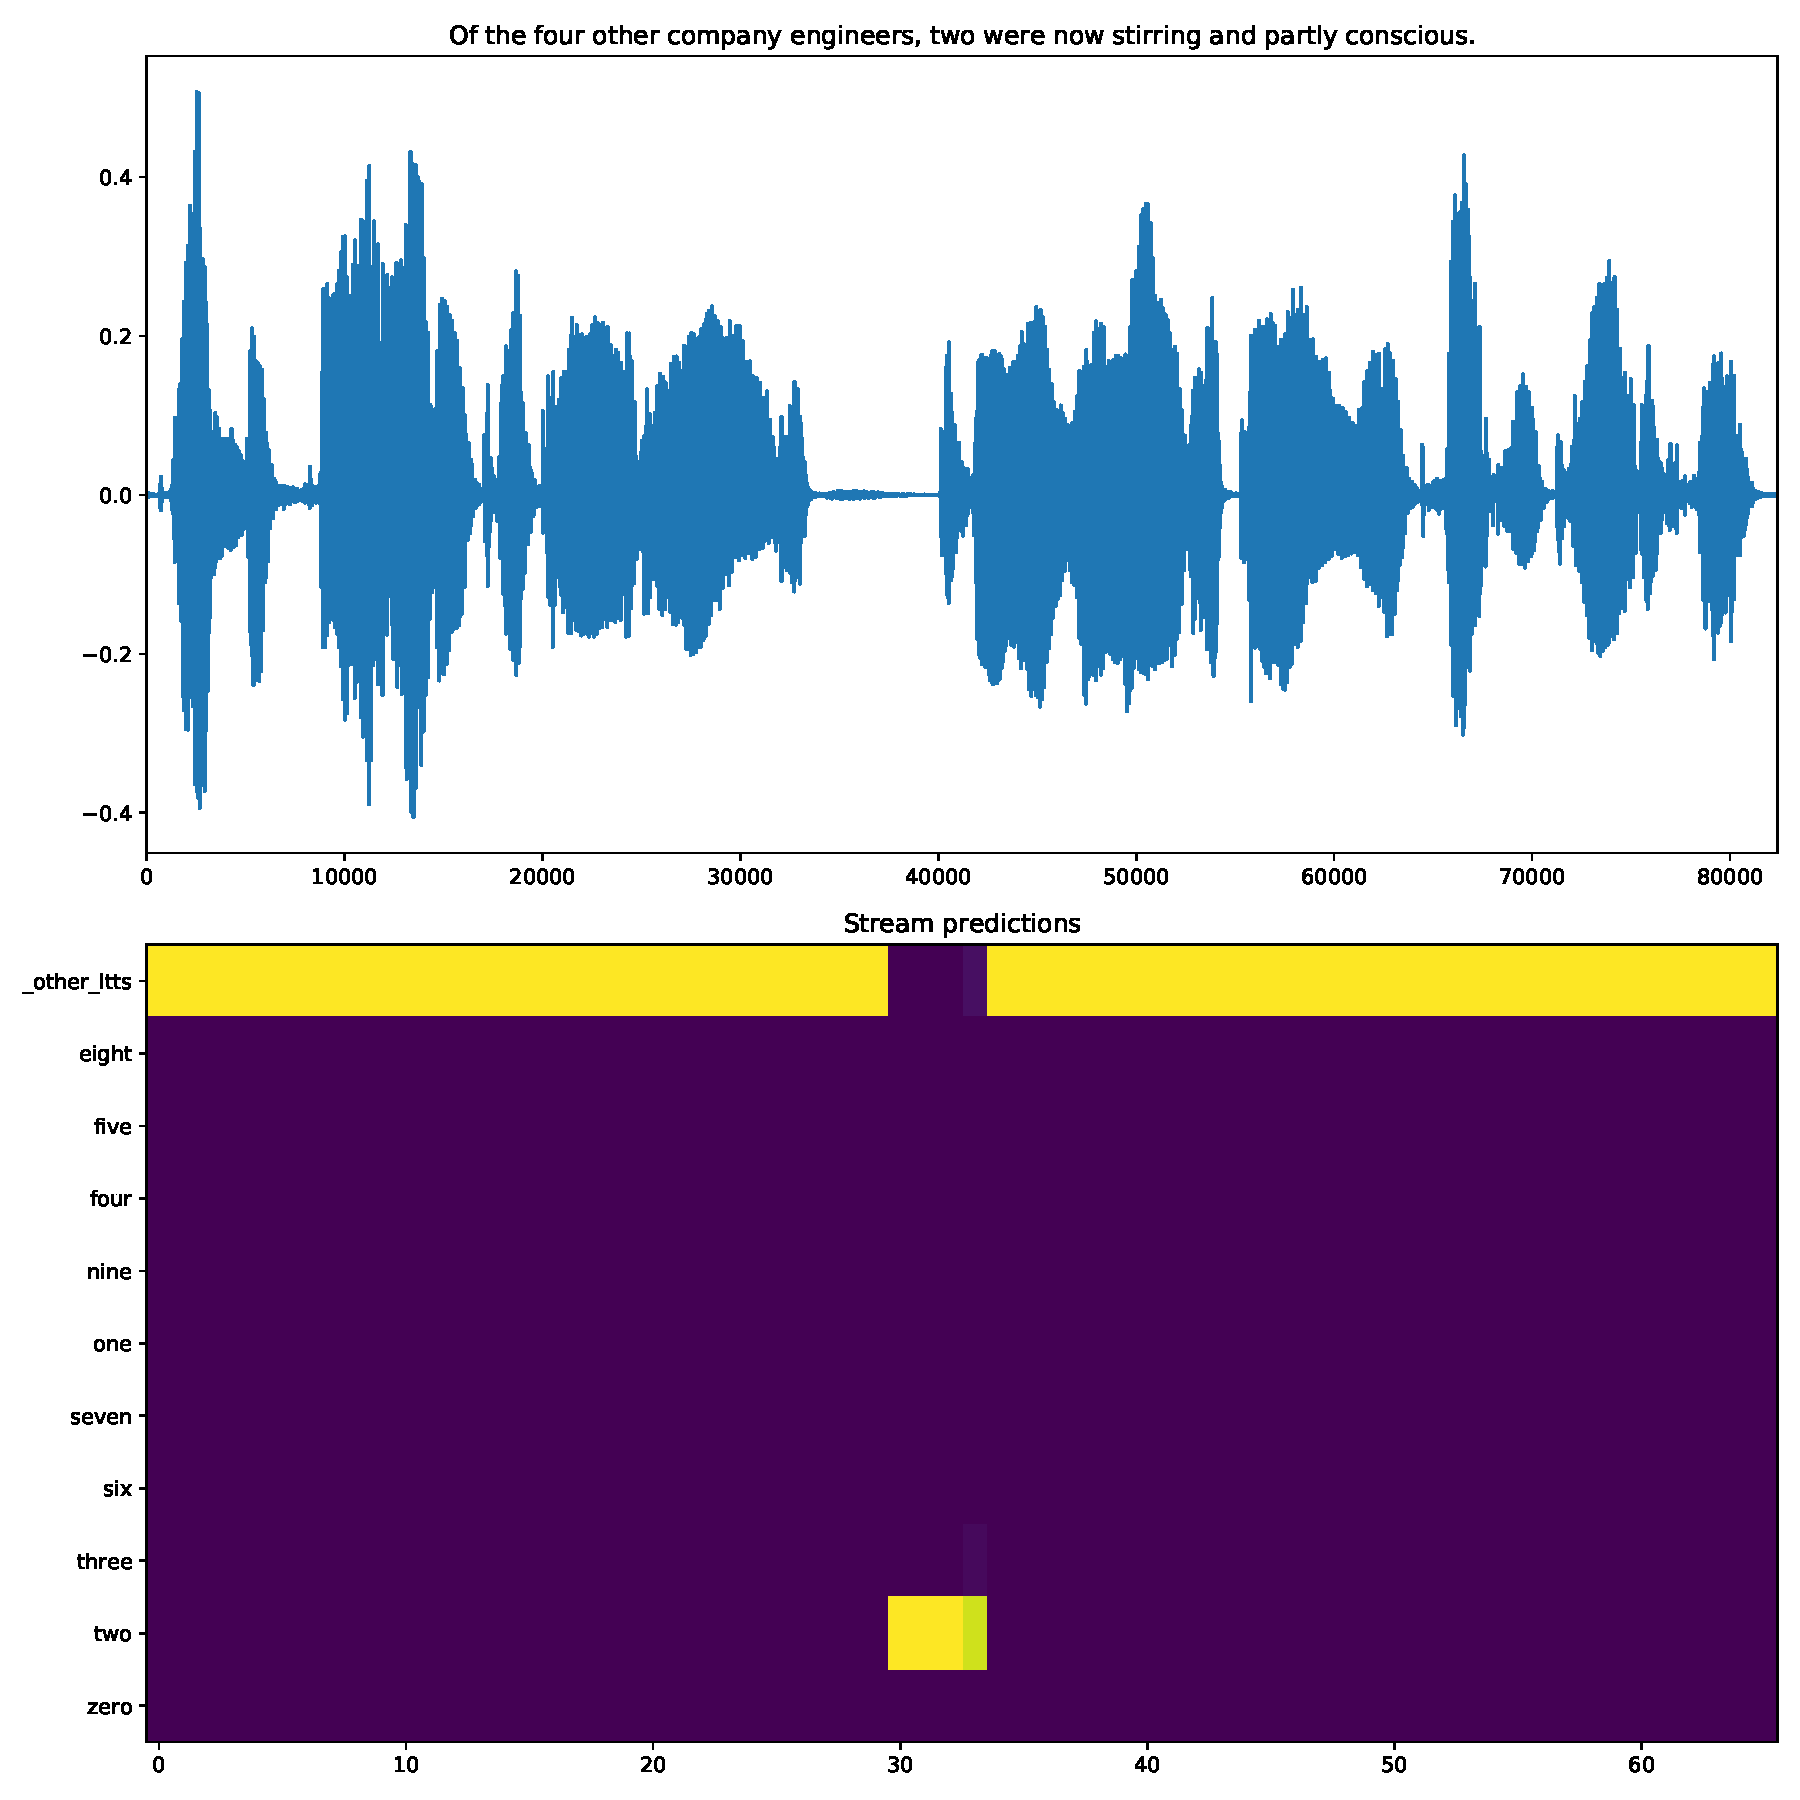
\includegraphics[width=0.9\linewidth]{stream_attention_ltts_mel04_LTnum_67.pdf}
    \caption{Stream 67 long words}%
    \label{fig:stream_attention_ltts_mel04_LTnum_67}
\end{figure}

\begin{figure}[h!]
    \centering
    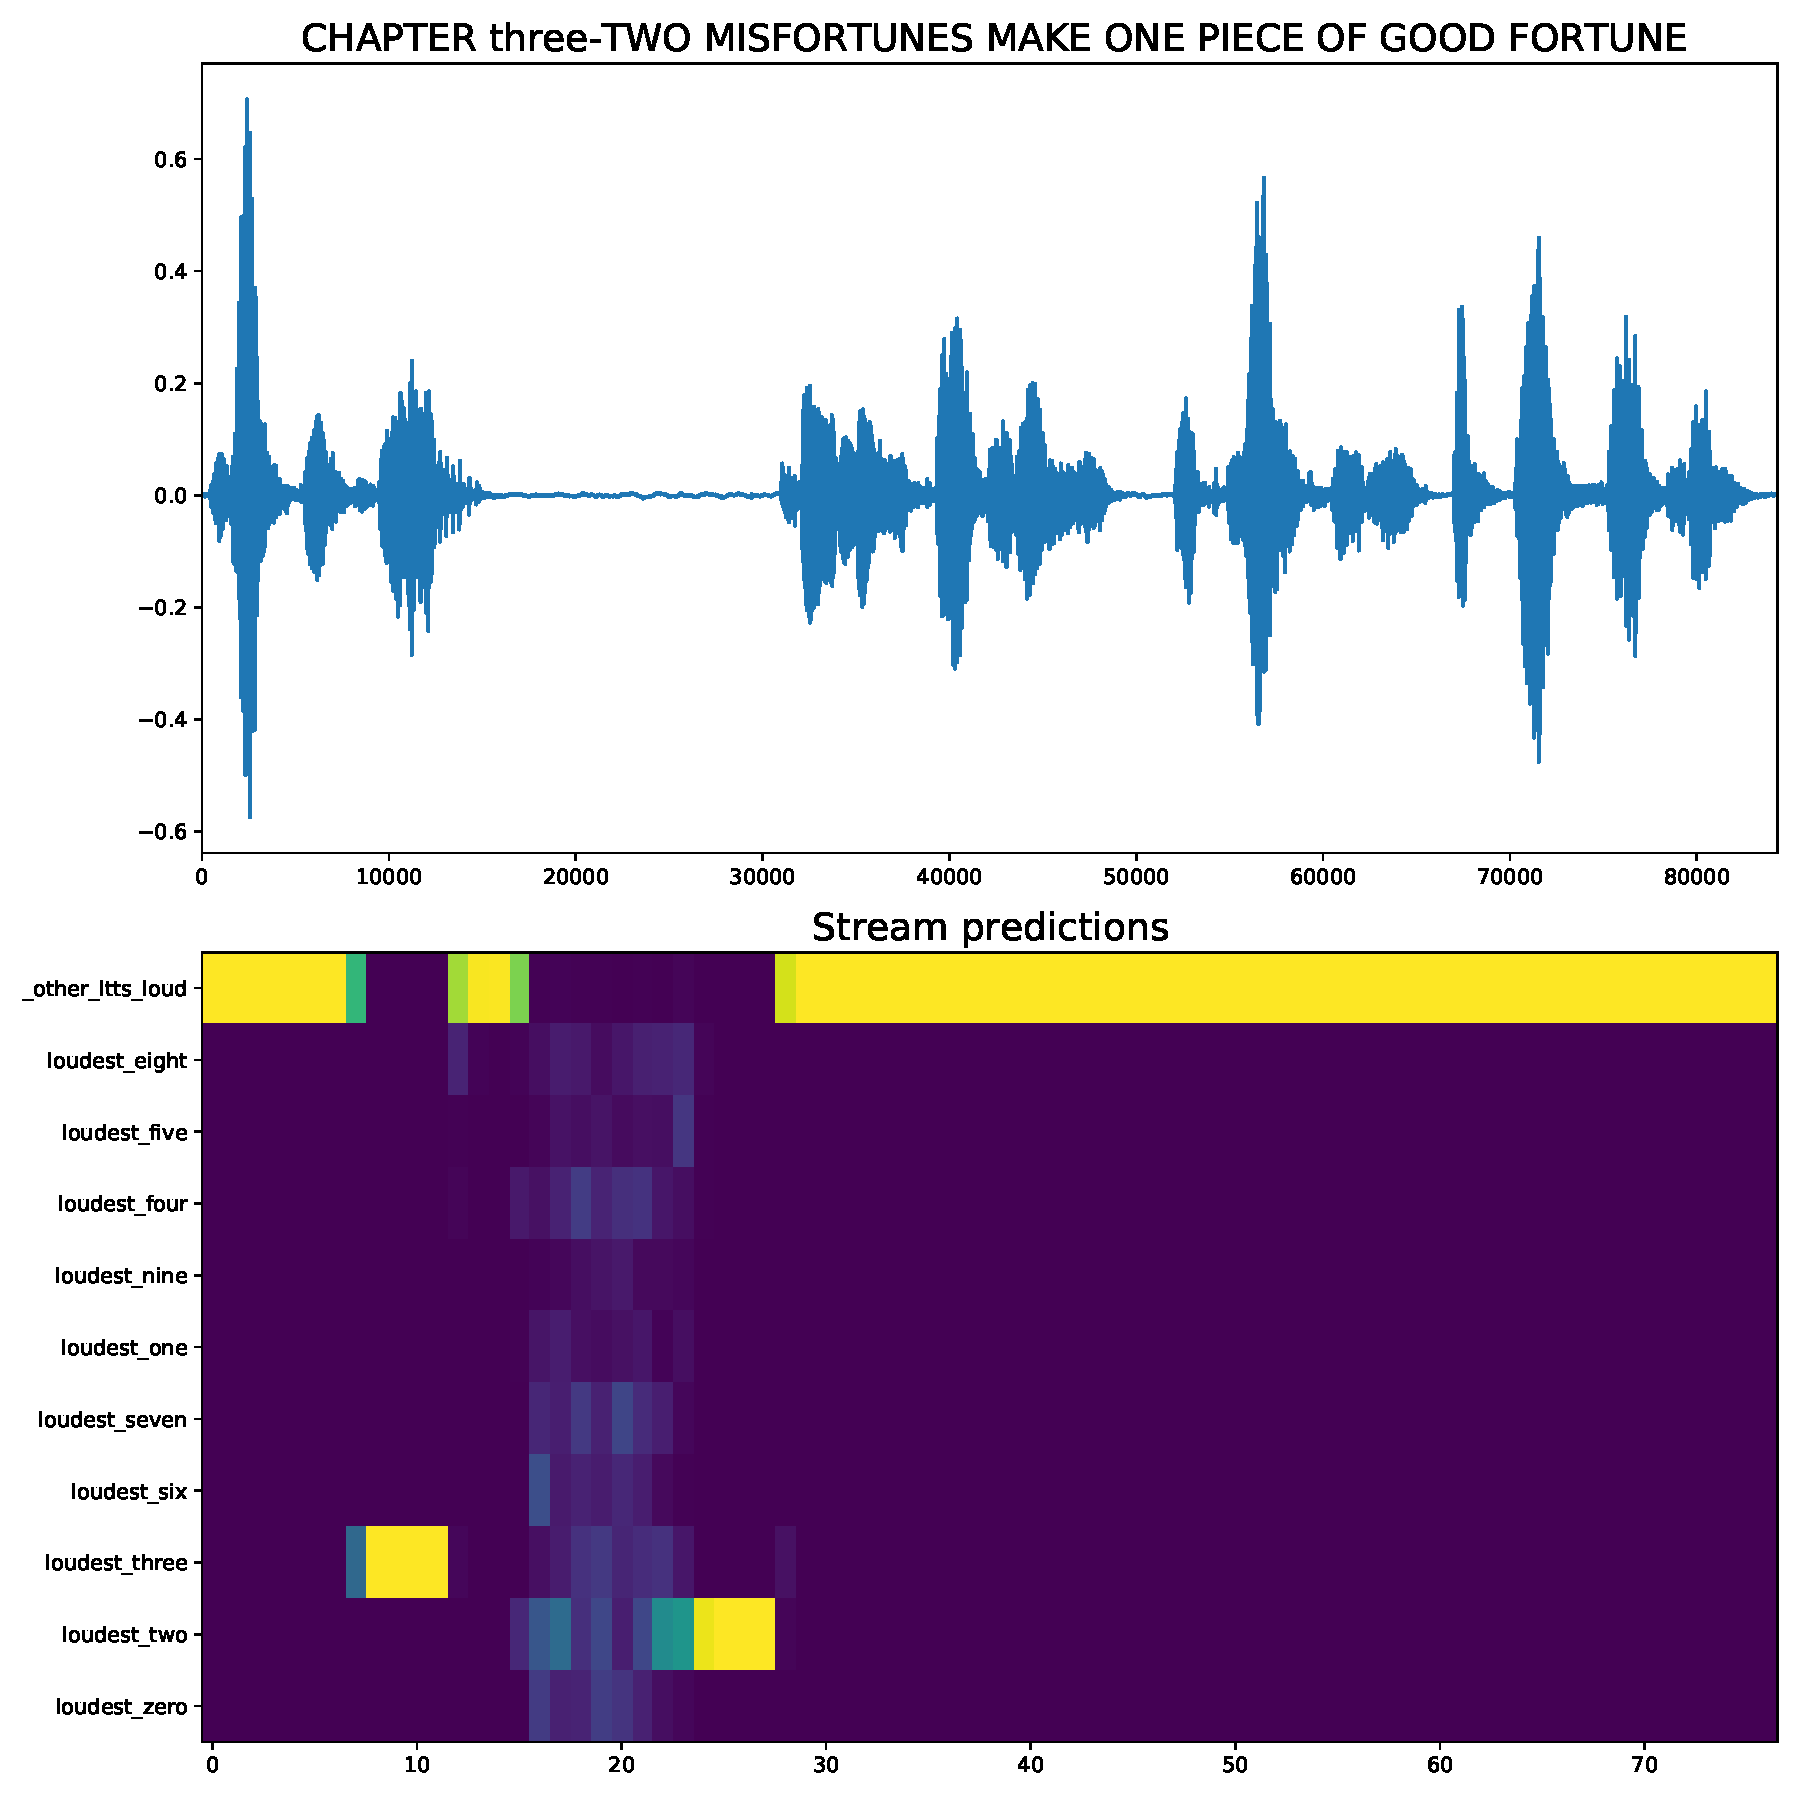
\includegraphics[width=0.9\linewidth]{stream2_attention_ltts_meL04_LTnumLS_19.pdf}
    \caption{Stream 19}%
    \label{fig:stream_attention_ltts_meL04_LTnumLS_19}
\end{figure}

% Attention vs Simple vs AreaNet vs VerticalAreaNet

TODO: Compare inference time, model size

TODO: Show stream with silence label

% Little difference in performance
